
%% bare_conf.tex
%% V1.3
%% 2007/01/11
%% by Michael Shell
%% See:
%% http://www.michaelshell.org/
%% for current contact information.
%%
%% This is a skeleton file demonstrating the use of IEEEtran.cls
%% (requires IEEEtran.cls version 1.7 or later) with an IEEE conference paper.
%%
%% Support sites:
%% http://www.michaelshell.org/tex/ieeetran/
%% http://www.ctan.org/tex-archive/macros/latex/contrib/IEEEtran/
%% and
%% http://www.ieee.org/

%%*************************************************************************
%% Legal Notice:
%% This code is offered as-is without any warranty either expressed or
%% implied; without even the implied warranty of MERCHANTABILITY or
%% FITNESS FOR A PARTICULAR PURPOSE! 
%% User assumes all risk.
%% In no event shall IEEE or any contributor to this code be liable for
%% any damages or losses, including, but not limited to, incidental,
%% consequential, or any other damages, resulting from the use or misuse
%% of any information contained here.
%%
%% All comments are the opinions of their respective authors and are not
%% necessarily endorsed by the IEEE.
%%
%% This work is distributed under the LaTeX Project Public License (LPPL)
%% ( http://www.latex-project.org/ ) version 1.3, and may be freely used,
%% distributed and modified. A copy of the LPPL, version 1.3, is included
%% in the base LaTeX documentation of all distributions of LaTeX released
%% 2003/12/01 or later.
%% Retain all contribution notices and credits.
%% ** Modified files should be clearly indicated as such, including  **
%% ** renaming them and changing author support contact information. **
%%
%% File list of work: IEEEtran.cls, IEEEtran_HOWTO.pdf, bare_adv.tex,
%%                    bare_conf.tex, bare_jrnl.tex, bare_jrnl_compsoc.tex
%%*************************************************************************

% *** Authors should verify (and, if needed, correct) their LaTeX system  ***
% *** with the testflow diagnostic prior to trusting their LaTeX platform ***
% *** with production work. IEEE's font choices can trigger bugs that do  ***
% *** not appear when using other class files.                            ***
% The testflow support page is at:
% http://www.michaelshell.org/tex/testflow/



% Note that the a4paper option is mainly intended so that authors in
% countries using A4 can easily print to A4 and see how their papers will
% look in print - the typesetting of the document will not typically be
% affected with changes in paper size (but the bottom and side margins will).
% Use the testflow package mentioned above to verify correct handling of
% both paper sizes by the user's LaTeX system.
%
% Also note that the "draftcls" or "draftclsnofoot", not "draft", option
% should be used if it is desired that the figures are to be displayed in
% draft mode.
%
\documentclass[10pt, conference, compsocconf]{IEEEtran}
% Add the compsocconf option for Computer Society conferences.
%
% If IEEEtran.cls has not been installed into the LaTeX system files,
% manually specify the path to it like:
% \documentclass[conference]{../sty/IEEEtran}





% Some very useful LaTeX packages include:
% (uncomment the ones you want to load)


% *** MISC UTILITY PACKAGES ***
%
%\usepackage{ifpdf}
% Heiko Oberdiek's ifpdf.sty is very useful if you need conditional
% compilation based on whether the output is pdf or dvi.
% usage:
% \ifpdf
%   % pdf code
% \else
%   % dvi code
% \fi
% The latest version of ifpdf.sty can be obtained from:
% http://www.ctan.org/tex-archive/macros/latex/contrib/oberdiek/
% Also, note that IEEEtran.cls V1.7 and later provides a builtin
% \ifCLASSINFOpdf conditional that works the same way.
% When switching from latex to pdflatex and vice-versa, the compiler may
% have to be run twice to clear warning/error messages.






% *** CITATION PACKAGES ***
%
%\usepackage{cite}
% cite.sty was written by Donald Arseneau
% V1.6 and later of IEEEtran pre-defines the format of the cite.sty package
% \cite{} output to follow that of IEEE. Loading the cite package will
% result in citation numbers being automatically sorted and properly
% "compressed/ranged". e.g., [1], [9], [2], [7], [5], [6] without using
% cite.sty will become [1], [2], [5]--[7], [9] using cite.sty. cite.sty's
% \cite will automatically add leading space, if needed. Use cite.sty's
% noadjust option (cite.sty V3.8 and later) if you want to turn this off.
% cite.sty is already installed on most LaTeX systems. Be sure and use
% version 4.0 (2003-05-27) and later if using hyperref.sty. cite.sty does
% not currently provide for hyperlinked citations.
% The latest version can be obtained at:
% http://www.ctan.org/tex-archive/macros/latex/contrib/cite/
% The documentation is contained in the cite.sty file itself.






% *** GRAPHICS RELATED PACKAGES ***
%
\ifCLASSINFOpdf
  % \usepackage[pdftex]{graphicx}
  % declare the path(s) where your graphic files are
  % \graphicspath{{../pdf/}{../jpeg/}}
  % and their extensions so you won't have to specify these with
  % every instance of \includegraphics
  % \DeclareGraphicsExtensions{.pdf,.jpeg,.png}
\else
  % or other class option (dvipsone, dvipdf, if not using dvips). graphicx
  % will default to the driver specified in the system graphics.cfg if no
  % driver is specified.
  % \usepackage[dvips]{graphicx}
  % declare the path(s) where your graphic files are
  % \graphicspath{{../eps/}}
  % and their extensions so you won't have to specify these with
  % every instance of \includegraphics
  % \DeclareGraphicsExtensions{.eps}
\fi
% graphicx was written by David Carlisle and Sebastian Rahtz. It is
% required if you want graphics, photos, etc. graphicx.sty is already
% installed on most LaTeX systems. The latest version and documentation can
% be obtained at: 
% http://www.ctan.org/tex-archive/macros/latex/required/graphics/
% Another good source of documentation is "Using Imported Graphics in
% LaTeX2e" by Keith Reckdahl which can be found as epslatex.ps or
% epslatex.pdf at: http://www.ctan.org/tex-archive/info/
%
% latex, and pdflatex in dvi mode, support graphics in encapsulated
% postscript (.eps) format. pdflatex in pdf mode supports graphics
% in .pdf, .jpeg, .png and .mps (metapost) formats. Users should ensure
% that all non-photo figures use a vector format (.eps, .pdf, .mps) and
% not a bitmapped formats (.jpeg, .png). IEEE frowns on bitmapped formats
% which can result in "jaggedy"/blurry rendering of lines and letters as
% well as large increases in file sizes.
%
% You can find documentation about the pdfTeX application at:
% http://www.tug.org/applications/pdftex





% *** MATH PACKAGES ***
%
%\usepackage[cmex10]{amsmath}
% A popular package from the American Mathematical Society that provides
% many useful and powerful commands for dealing with mathematics. If using
% it, be sure to load this package with the cmex10 option to ensure that
% only type 1 fonts will utilized at all point sizes. Without this option,
% it is possible that some math symbols, particularly those within
% footnotes, will be rendered in bitmap form which will result in a
% document that can not be IEEE Xplore compliant!
%
% Also, note that the amsmath package sets \interdisplaylinepenalty to 10000
% thus preventing page breaks from occurring within multiline equations. Use:
%\interdisplaylinepenalty=2500
% after loading amsmath to restore such page breaks as IEEEtran.cls normally
% does. amsmath.sty is already installed on most LaTeX systems. The latest
% version and documentation can be obtained at:
% http://www.ctan.org/tex-archive/macros/latex/required/amslatex/math/





% *** SPECIALIZED LIST PACKAGES ***
%
%\usepackage{algorithmic}
% algorithmic.sty was written by Peter Williams and Rogerio Brito.
% This package provides an algorithmic environment fo describing algorithms.
% You can use the algorithmic environment in-text or within a figure
% environment to provide for a floating algorithm. Do NOT use the algorithm
% floating environment provided by algorithm.sty (by the same authors) or
% algorithm2e.sty (by Christophe Fiorio) as IEEE does not use dedicated
% algorithm float types and packages that provide these will not provide
% correct IEEE style captions. The latest version and documentation of
% algorithmic.sty can be obtained at:
% http://www.ctan.org/tex-archive/macros/latex/contrib/algorithms/
% There is also a support site at:
% http://algorithms.berlios.de/index.html
% Also of interest may be the (relatively newer and more customizable)
% algorithmicx.sty package by Szasz Janos:
% http://www.ctan.org/tex-archive/macros/latex/contrib/algorithmicx/




% *** ALIGNMENT PACKAGES ***
%
%\usepackage{array}
% Frank Mittelbach's and David Carlisle's array.sty patches and improves
% the standard LaTeX2e array and tabular environments to provide better
% appearance and additional user controls. As the default LaTeX2e table
% generation code is lacking to the point of almost being broken with
% respect to the quality of the end results, all users are strongly
% advised to use an enhanced (at the very least that provided by array.sty)
% set of table tools. array.sty is already installed on most systems. The
% latest version and documentation can be obtained at:
% http://www.ctan.org/tex-archive/macros/latex/required/tools/


%\usepackage{mdwmath}
%\usepackage{mdwtab}
% Also highly recommended is Mark Wooding's extremely powerful MDW tools,
% especially mdwmath.sty and mdwtab.sty which are used to format equations
% and tables, respectively. The MDWtools set is already installed on most
% LaTeX systems. The lastest version and documentation is available at:
% http://www.ctan.org/tex-archive/macros/latex/contrib/mdwtools/


% IEEEtran contains the IEEEeqnarray family of commands that can be used to
% generate multiline equations as well as matrices, tables, etc., of high
% quality.


%\usepackage{eqparbox}
% Also of notable interest is Scott Pakin's eqparbox package for creating
% (automatically sized) equal width boxes - aka "natural width parboxes".
% Available at:
% http://www.ctan.org/tex-archive/macros/latex/contrib/eqparbox/





% *** SUBFIGURE PACKAGES ***
%\usepackage[tight,footnotesize]{subfigure}
% subfigure.sty was written by Steven Douglas Cochran. This package makes it
% easy to put subfigures in your figures. e.g., "Figure 1a and 1b". For IEEE
% work, it is a good idea to load it with the tight package option to reduce
% the amount of white space around the subfigures. subfigure.sty is already
% installed on most LaTeX systems. The latest version and documentation can
% be obtained at:
% http://www.ctan.org/tex-archive/obsolete/macros/latex/contrib/subfigure/
% subfigure.sty has been superceeded by subfig.sty.



%\usepackage[caption=false]{caption}
%\usepackage[font=footnotesize]{subfig}
% subfig.sty, also written by Steven Douglas Cochran, is the modern
% replacement for subfigure.sty. However, subfig.sty requires and
% automatically loads Axel Sommerfeldt's caption.sty which will override
% IEEEtran.cls handling of captions and this will result in nonIEEE style
% figure/table captions. To prevent this problem, be sure and preload
% caption.sty with its "caption=false" package option. This is will preserve
% IEEEtran.cls handing of captions. Version 1.3 (2005/06/28) and later 
% (recommended due to many improvements over 1.2) of subfig.sty supports
% the caption=false option directly:
%\usepackage[caption=false,font=footnotesize]{subfig}
%
% The latest version and documentation can be obtained at:
% http://www.ctan.org/tex-archive/macros/latex/contrib/subfig/
% The latest version and documentation of caption.sty can be obtained at:
% http://www.ctan.org/tex-archive/macros/latex/contrib/caption/




% *** FLOAT PACKAGES ***
%
%\usepackage{fixltx2e}
% fixltx2e, the successor to the earlier fix2col.sty, was written by
% Frank Mittelbach and David Carlisle. This package corrects a few problems
% in the LaTeX2e kernel, the most notable of which is that in current
% LaTeX2e releases, the ordering of single and double column floats is not
% guaranteed to be preserved. Thus, an unpatched LaTeX2e can allow a
% single column figure to be placed prior to an earlier double column
% figure. The latest version and documentation can be found at:
% http://www.ctan.org/tex-archive/macros/latex/base/



%\usepackage{stfloats}
% stfloats.sty was written by Sigitas Tolusis. This package gives LaTeX2e
% the ability to do double column floats at the bottom of the page as well
% as the top. (e.g., "\begin{figure*}[!b]" is not normally possible in
% LaTeX2e). It also provides a command:
%\fnbelowfloat
% to enable the placement of footnotes below bottom floats (the standard
% LaTeX2e kernel puts them above bottom floats). This is an invasive package
% which rewrites many portions of the LaTeX2e float routines. It may not work
% with other packages that modify the LaTeX2e float routines. The latest
% version and documentation can be obtained at:
% http://www.ctan.org/tex-archive/macros/latex/contrib/sttools/
% Documentation is contained in the stfloats.sty comments as well as in the
% presfull.pdf file. Do not use the stfloats baselinefloat ability as IEEE
% does not allow \baselineskip to stretch. Authors submitting work to the
% IEEE should note that IEEE rarely uses double column equations and
% that authors should try to avoid such use. Do not be tempted to use the
% cuted.sty or midfloat.sty packages (also by Sigitas Tolusis) as IEEE does
% not format its papers in such ways.





% *** PDF, URL AND HYPERLINK PACKAGES ***
%
%\usepackage{url}
% url.sty was written by Donald Arseneau. It provides better support for
% handling and breaking URLs. url.sty is already installed on most LaTeX
% systems. The latest version can be obtained at:
% http://www.ctan.org/tex-archive/macros/latex/contrib/misc/
% Read the url.sty source comments for usage information. Basically,
% \url{my_url_here}.





% *** Do not adjust lengths that control margins, column widths, etc. ***
% *** Do not use packages that alter fonts (such as pslatex).         ***
% There should be no need to do such things with IEEEtran.cls V1.6 and later.
% (Unless specifically asked to do so by the journal or conference you plan
% to submit to, of course. )


% correct bad hyphenation here
\usepackage{cite}
\usepackage{graphicx}
\usepackage[cmex10]{amsmath}
\usepackage{algpseudocode}
\usepackage{algorithm}
\renewcommand{\algorithmicrequire}{\textbf{Input:}}
\renewcommand{\algorithmicensure}{\textbf{Output:}}
\usepackage{subfigure}
\usepackage{listings}

\newtheorem{theorem}{Theorem}
\newtheorem{lemma}[theorem]{Lemma}
\newtheorem{corollary}[theorem]{Corollary}
\newtheorem{remark}[theorem]{Remark}
\newtheorem{definition}[theorem]{Definition}
\newtheorem{equat}[theorem]{Equation}
\newtheorem{example}[theorem]{Example}
\newtheorem{property}[theorem]{Property}

\newcommand\clustream{\emph{CluStream}}
\newcommand\our{\emph{CluStream-Spark}}

\usepackage{color}
\usepackage{amssymb}
\usepackage{graphicx}
%\usepackage{bbm}
\usepackage{subfigure}
\usepackage{ifthen}
\usepackage{url}
\usepackage{verbatim}
\usepackage[ansinew]{inputenc}

\usepackage{caption}



\begin{document}
%
% paper title
% can use linebreaks \\ within to get better formatting as desired
\title{Scalable Online-Offline Stream Clustering in Apache Spark}


% author names and affiliations
% use a multiple column layout for up to two different
% affiliations

\author{\IEEEauthorblockN{Omar Backhoff}
\IEEEauthorblockA{%Computational Science and Engineering\\
Technische Universit\"{a}t M\"{u}nchen (TUM)\\
Munich, Germany\\
omarbackhoff@gmail.com}
\and
\IEEEauthorblockN{Eirini Ntoutsi}
\IEEEauthorblockA{%Faculty of Electrical Engineering and Computer Science\\
Leibniz Universit\"{a}t Hannover\\
Hanover, Germany\\
ntoutsi@kbs.uni-hannover.de
}
}
% conference papers do not typically use \thanks and this command
% is locked out in conference mode. If really needed, such as for
% the acknowledgment of grants, issue a \IEEEoverridecommandlockouts
% after \documentclass

% for over three affiliations, or if they all won't fit within the width
% of the page, use this alternative format:
% 
%\author{\IEEEauthorblockN{Michael Shell\IEEEauthorrefmark{1},
%Homer Simpson\IEEEauthorrefmark{2},
%James Kirk\IEEEauthorrefmark{3}, 
%Montgomery Scott\IEEEauthorrefmark{3} and
%Eldon Tyrell\IEEEauthorrefmark{4}}
%\IEEEauthorblockA{\IEEEauthorrefmark{1}School of Electrical and Computer Engineering\\
%Georgia Institute of Technology,
%Atlanta, Georgia 30332--0250\\ Email: see http://www.michaelshell.org/contact.html}
%\IEEEauthorblockA{\IEEEauthorrefmark{2}Twentieth Century Fox, Springfield, USA\\
%Email: homer@thesimpsons.com}
%\IEEEauthorblockA{\IEEEauthorrefmark{3}Starfleet Academy, San Francisco, California 96678-2391\\
%Telephone: (800) 555--1212, Fax: (888) 555--1212}
%\IEEEauthorblockA{\IEEEauthorrefmark{4}Tyrell Inc., 123 Replicant Street, Los Angeles, California 90210--4321}}




% use for special paper notices
%\IEEEspecialpapernotice{(Invited Paper)}




% make the title area
\maketitle


\begin{abstract}
Two of the most popular strategies to mine big data are distributed comput-
ing and stream mining. The purpose of this thesis is to incorporate both together
bringing a competitive stream clustering method into a modern framework for
distributed computing, namely, Apache Spark. The method in question is CluS-
tream, a stream clustering method which separates the clustering process into two
different phases: an online phase which handles the incoming stream, generating
statistical summaries of the data and an offline phase which takes those summaries
to generate the final clusters. These summaries also contain valuable information
which can be used for further analysis. The main goal is to adapt this method in
such a framework in order to obtain a scalable stream clustering method which is
open source and can be used by the Apache Spark community.
\end{abstract}

\begin{IEEEkeywords}
big data streams; stream mining; stream clustering; CluStream
\end{IEEEkeywords}


% For peer review papers, you can put extra information on the cover
% page as needed:
% \ifCLASSOPTIONpeerreview
% \begin{center} \bfseries EDICS Category: 3-BBND \end{center}
% \fi
%
% For peerreview papers, this IEEEtran command inserts a page break and
% creates the second title. It will be ignored for other modes.
\IEEEpeerreviewmaketitle


%-------------------------------------------------------------
\section{Introduction}
\label{sec:intro}
The analysis of data streams comes along with important questions: what kind of
data is it? What important information is contained in it? How does the stream
evolve? The key question for this project among those is the latter, i.e. dealing with
the evolution of the stream, because prior to the development of the CluStream \cite{clustreamOrig}
method there was not an easy to answer that question as it was one of the first to
tackle this issue.

Clustering is one of the main tasks in data mining, also often referred as an
exploratory subtask of it. As the name implies, the objective is to find clusters, i.e.,
collections of objects that share common properties. One can also relate this task
to unsupervised machine learning, which intends to classify data when it lacks of
labels, i.e., when the data instance does not indicate to which category it belongs.
The CluStream method was developed in 2003 \cite{clustreamOrig} and its main purpose is to pro-
vide more information than previously developed algorithms for data stream clus-
tering by that time. It provides a solution for handling streams of data indepen-
dently from the one that finds the final clusters. It consists of two phases (passes)
instead of one; the first one deals with the incoming data and stores relevant in-
formation over time and the second one is in charge of the clustering using the
previously generated information. In other words,

% For each batch of data, statistically relevant �summaries� of the data are created and stored at a defined pace. This storing pace follows a specific storage scheme such that the disk space requirement reduces drastically; this is necessary as in most cases for data streams one does not want to store everything
% that arrives, one reason being the big data requires large and expensive computational resources (processing power and storage).
% On user demand, the stored �summaries can be used for the end clustering
% task as they include all necessary information to achieve accurate results.
% Additionally, as these summaries are stored over time, a user defined time
% horizon/window can be chosen in order to analyze the data in different time
% periods, giving the possibility of a better understanding of the evolution of
% the data.


%-------------------------------------------------------------
\section{Related Work}


% \subsection{SAMOA}
\textit{CluStream} has been implemented in different types of software and libraries, being \textit{SAMOA - Scalable Advanced Massive Online Analysis} one of the options. It is also a distributed computing implementation of the algorithm. The difference is that it is not implemented in \textit{Spark}, but rather in a \textit{Distributed Stream Processing Engine} which adapts the \textit{MapReduce} approach to parallel stream processing\cite{samoa}.

Main differences with this adaptation: 

\begin{itemize}
 \item It does not include an offline macro-clustering phase.
 \item It is developed in \textit{Java} and not designed to work with Spark.
\end{itemize}

% \subsection{StreamDM}
\textit{StreamDM} is a collection of algorithms for mining big data streams \footnote{As it is stated by them here: http://huawei-noah.github.io/streamDM/}. One of the included methods for stream clustering is \textit{CluStream}. This collection of algorithms is developed for Spark.

Main differences with this adaptation: 

\begin{itemize}
 \item It does not include an offline macro-clustering phase.
\end{itemize}

%-------------------------------------------------------------
\section{Basic concepts}
\label{sec:basics}
\subsection{CluStream}

\textit{CluStream} is a method developed in the Watson Research Center at IBM and the University of Illinois, UIUC. This method presented a different approach on the matter of clustering streams of data with respect to a modified version of \textit{K-Means} which was adapted to work also with data streams. The main difference relies on the separation of the clustering process into two parts: one which would handle the data stream itself gathering only statistically relevant information (online part) and another which actually process the results of the former to produce the actual clusters wanted (offline part). 

Separating the clustering process provides the user several advantages, among others:

\begin{itemize}
 \item by saving only statistical data, rather than the original content, it is possible to save physical storage space (e.g. hard drive space) and therefore reducing costs and allowing a wider range in time to be clustered.
 
 \item The method also allows the analysis of the evolution of the data, as the necessary information for that is contained in the stored statistical information.
 
 \item Because the two parts operate independently it allows the user to select a time horizon, or even a time window, to perform the offline clustering part using the stored statistical information.
\end{itemize}

\subsubsection{The CluStream framework}

This method is built over a few ideas that need to be conceptualized, which will answer fundamental questions and set up a basis of terminology useful along this work.

\begin{itemize}
 \item \textbf{Micro-Clusters}: that is the given name for the statistical information summaries that is computed during the online component. They are a temporal extension of \textit{cluster feature vectors}\cite{zhang96birch}, which benefit from an additive feature that makes them a natural choice for the data stream problem\cite{clustreamOrig}.
 
 \item \textbf{Pyramidal time frame}: micro-clusters are stored periodically following a pyramidal pattern. This allows a nice tradeoff between the ability to store large amounts of information while giving the user the possible to work with different time horizons without loosing too much precision. The statistical summaries stored are used by the offline component to compute finally the macro-clusters which are the actual clusters the user intended to get.
\end{itemize}


\subsubsection{Maintaining the micro-clusters}

Whenever a new point arrives, it is necessary to find its nearest micro-cluster. It is possible to calculate an average radious or \textit{RMSD}, only to then compare the distance to the point to a factor of it: when the distance between a point and its nearest micro-cluster is smaller or equal to the average radiuos (of the micro-cluster in question) times a user defined factor, then this point is added to the micro-cluster. Adding a point to a micro-cluster means that the properties of the micro-cluster change, such as RMSD and size (number of points).

Whenever a point (outlier) does not fulfill the mentioned condition, then a new micro-cluster has to be created in order to give this point a chance as a potential new cluster. In order to do so, an older micro-cluster has to be deleted or two micro-clusters have to be merged. To determine which solution is appropriate a recency value for each micro-cluster has to be determined\footnote{See \cite{clustreamOrig} for more details.} and until all the micro-clusters which have an older recency value than a user specified parameter are deleted, it is possible to start merging the micro-clusters which are closest to one another.

\subsubsection{Offline macro-clusterig}

The macro-clustering part is done by selecting a time window and then performing a modified version of \textit{K-Means} to cluster the center of the current micro-clusters using the size as weights. 

\subsection{SPARK}
\textit{Apache Spark} is an open source framework developed in the AMPLab at the University of California.
Traditionally, MapReduce and DAG engines are based on an acyclic data flow, which makes them non optimal for these applications listed above. In this flow, data has to be read from a stable storage system, like a distributed file system, and then processed on a series of jobs only to be written back to the stable storage. This process of reading and writing data on each step of the workflow causes a significant rise in computational cost.

The solution proposed offers \textit{resilient distributed datasets (RDDs)} to overcome this issue efficiently. RDDs are stored in memory between queries (no need of replication) and they can rebuild themselves in case of failure as they remember how they were originally built from other datasets by transformations such as \textit{map, group, join}.

\subsection{SPARK streaming}

\begin{figure}[h!]
 \centering
 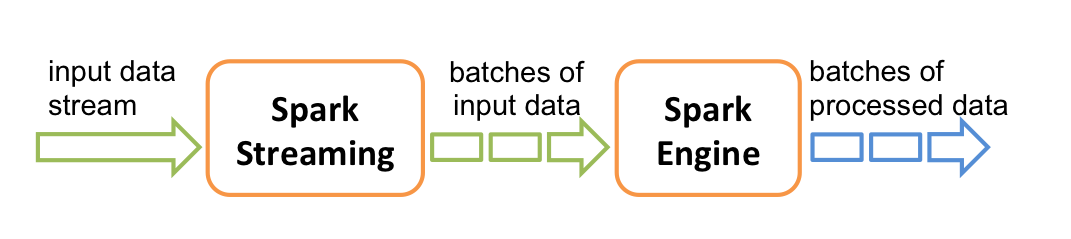
\includegraphics[scale=0.45]{./styles/streaming-flow.png}
 % streaming-flow.png: 0x0 pixel, 300dpi, 0.00x0.00 cm, bb=
 \caption{Flow of data in Spark streaming}
 \label{fig:streamFlow}
\end{figure}

Figure \ref{fig:streamFlow} shows the general idea of Spark streaming\cite{sparkStreaming}, a raw stream is linked to this module and it converts it to batches of data at user-defined intervals. These batches of data are then treated as RDDs, thus it gets distributed over the cluster where Spark runs. The abstraction of a data stream in Spark is called \textit{DStream}, which stands for Discretized Stream, and is continuous series of RDDs. In a \textit{DStream}, each RDD contains data from a specific interval of time, as it can be seen in Figure \ref{fig:dstream}.


\begin{figure}[h!]
 \centering
 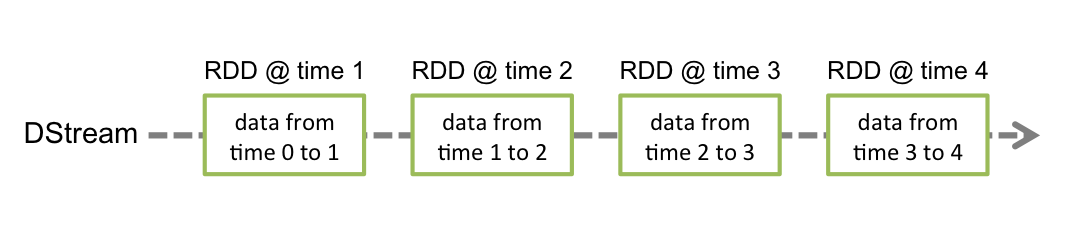
\includegraphics[scale=0.45]{./styles/streaming-dstream.png}
 % streaming-flow.png: 0x0 pixel, 300dpi, 0.00x0.00 cm, bb=
 \caption{DStreams are Spark streaming's abstraction of a data stream}
 \label{fig:dstream}
\end{figure}



%-------------------------------------------------------------
\section{CluStream extension in Apache SPARK}
\label{sec:our}
There are some modifications which had to be done in order to adapt \textit{CluStream} in Spark. Working with Spark means worrking distributed computing and, thus, the algorithm has to be able to work in parallel. Both parts (online and offline) were adapted.

\subsection{CluStreamOnline class (online phase)}

Two processes were modified: processing the stream and updating the micro-clusters. As this adaptation uses Spark Streaming, the points coming from the stream are processed in batches at user specified time intervals. This contrasts with the original methodology which indicates to process point by point. The main difference with the batch processing method is that now points laying in current micro-clusters are processed before than the ones that are not, this also includes updating the micro-clusters before processint the points laying out. The reason for this is that as part of the strategy chosen to parallelize the algorithm, the micro-clusters are maintained locally and processing the outliers is also performed locally because deleting and merging requires to modify the micro-clusters for every point.

\subsubsection{Finding nearest micro-cluster}

The maintenance of the micro-clusters starts with this operation. After initialization (described in \cite{clustreamOrig}) is performed, finding the nearest micro-clusters for all the points is the very first thing to be done for every new batch of data.

\begin{algorithm}
 \caption{Find nearest micro-cluster.}\label{alg:assign}
 \begin{algorithmic}[1]
  \Require{\textit{rdd: RDD[breeze.linalg.Vector[Double]], mcInfo: Array[(McI,Int)]}| \textit{rdd} is an RDD containing data points and \textit{mcInfo} is the collection of the micro-clusters information.} 
  \Ensure{\textit{rdd: RDD[(Int, breeze.linalg.Vector[Double])]} | returns a tuple of the point itself and the unique ID of the nearest micro-cluster.}
  \vspace{10pt}
  \ForAll {$p \in rdd$}
  \State $minDistance \gets Double.PositiveInfinity$
  \State $minIndex \gets Int.MaxValue$
  \ForAll {$mc \in mcInfo$}
  \State $distance \gets squaredDistance(p, mc_1.centroid)$
  \If {$distance \leq minDistance$}
  \State $minDistance \gets distance$
  \State $minIndex \gets mc_2$
  \EndIf
  \EndFor
  \State $p = (minIndex,p)$
  \EndFor
  \Return $rdd$
 \end{algorithmic}
\end{algorithm}

Finding the nearest micro-clusters is an operation of complexity $O(n*q*d)$, where $n$ is the number of points, $q$ the number of micro-clusters and $d$ the dimension of the points; $q$ and $d$ remain constant during runtime but $n$ might vary. Algorithm \ref{alg:assign} describes a simple search for the minimum distance for every point in the RDD to the micro-clusters. This is also a good opportunity to show how this works using Spark and \textit{Scala}:

\
\begin{lstlisting}[language=Scala, tabsize=2, breaklines=true,basicstyle=\footnotesize,frame=lines,numbers=left]
def assignToMicroCluster(rdd: RDD[Vector[Double]], mcInfo: Array[(MicroClusterInfo, Int)]): RDD[(Int, Vector[Double])] = {
    rdd.map { a =>
      var minDist = Double.PositiveInfinity
      var minIndex = Int.MaxValue
      for (mc <- mcInfo) {
        val dist = squaredDistance(a, mc._1.centroid)
        if (dist < minDist) {
          minDist = dist
          minIndex = mc._2
        }}
      (minIndex, a)
    }}
\end{lstlisting}

\textit{Scala} allows operating the elements of a collection, e.g. an array, through a map operation. The code above represents the actual function in the source code of this project that does what Algorithm \ref{alg:assign} says for the initialization process. The variable $mcInfo$ contains a summarized information taken from the micro-clusters; this variable is broadcasted to always have updated information for each batch. In this programming language, the last line defines what the function returns; it can be seen in line 2 of the mentioned function that there is actually only one instruction called, and that is $rdd.map\{a => function(a) \}$. This operation, \textit{map}, requires a function to be passed, which at the same time receives as argument each element $a$ of a collection, in this case the collection is $rdd$, and returns anything resulting from that function which will replace $a$. In other words, it is possible to operate and change every element of a collection through $map$ with a specified function and get a new "updated" collection in return.

To find the nearest micro-cluster of a point, in this case $a$, an iterative process is used, which computes the squared distance from $a$ to all micro-clusters' cetroids and stores only smaller distances and the unique ID of such so-far-nearest micro-cluster. When the iteration finishes, the function returns the tuple $(minIndex,a)$ which replaces the element $a$.

Spark uses this $map$ operation to serialize the function passed so that all nodes in the cluster get the same instruction, this is exactly how computations are parallelized  within this framework. At this point, every node performs this operation to find the nearest micro-cluster for all the points they locally have.



\subsubsection{Processing points}\label{procpoints}

The points are separated in two: points within micro-clusters and outliers, it is possible to compute the necessary information from them to update the micro-clusters. It is important to perform this step before handling the outliers because this adaptation process the points for batches of data and not points individually as they arrive, and the reasons are:

\begin{itemize}
 \item Every point for a batch is treated equally in terms of temporal properties. A batch of points gets distributed among the cluster and they all get the same time stamp. As the points are processed in parallel, and there is no constant communication among nodes, there is no reason to assume that a point is older or newer within that batch because then race conditions would occur resulting in unpredictable results.
\item Taking into account the previous statement, the process of handling outliers involve deleting and merging micro-clusters and not processing the points first would lead to invalid assignations as some micro-clusters might not exist anymore or might have changed while being merged.
\end{itemize}

These two points are some of the key differences between the original $CluStream$ method and this adaptation. For the original, it is possible to handle point by point as each have different clear time stamps.

Processing the points means two things: to compute the values required to update the micro-clusters, i.e. the \textit{cluster feature vector}, and actually updating the micro-clusters. This is another good opportunity to show a piece of code because it will be important for the performance analysis later on, and also to show how it is possible to reduce the amount of code needed for such operation. First, computing the \textit{cluster feature vector}:

\
\begin{lstlisting}[language=Scala, tabsize=2, breaklines=true,basicstyle=\footnotesize,frame=lines,numbers=left]
val aggregateFunction = 
  (aa: (Vector[Double], Vector[Double], Long), 
  bb: (Vector[Double], Vector[Double], Long)) =>                     
  (aa._1 :+ bb._1, aa._2 :+ bb._2, aa._3 + bb._3)
		
val sumsAndSumsSquares = 
  dataIn.mapValues(v => (v, v :* v, 1L))
    .reduceByKey(aggregateFunction).collect()
\end{lstlisting}

First a function called $aggregateFunction$ is defined, and this is a generic function that can get passed as an argument to another function. It has the purpose of taking any two given values, in this case two given tuples, and return a tuple that contains the sum of every element of one tuple with the respective element of the other tuple: 

\begin{gather*}
aggregateFunction =  ((v_1 , u_1 , k_1 ) ,  (v_2 , u_2 , k_2 )) => \\
(v_1 + v_2 , u_1 + u_2 , k_1 + k_2) 
\end{gather*}


From the assignation process, the points that are going to be processed are located in $dataIn$, which looks as follows:

$$dataIn=\{(id_1,p_1),(id_2,p_2),...\},$$ 
where, $id_i$ is the unique identifier of the micro-cluster the point $p_i$ belongs to. Then a $map$ is performed only on the "values" of the tuple, considering that Spark can interpret tuples as $(key,value)$ pairs, to replace each point $p_i$ with a tuple containing $p_i$, squared elements of $p_i$ and the \textit{Long} value of 1: 

\begin{gather*}
dataIn.mapValues( v => (v, v * v, 1) ) = \\
\{ (id_1, (p_1 , p_1^T I p_1 , 1) ) , (id_2 , (p_2 , p_2^T I p_2 , 1) ) ,... \}
\end{gather*}

To square the elements means to element-wise square the values of a vector $v$, therefore this is represented by $v^TIv$. This is done in order to perform a $reduceByKey$ operation, which is how Spark combines and operates the distributed elements of an RDD:

$$dataIn.mapValues(...).reduceByKey(aggregateFunction) =$$
$$\{ (id_1, (p_{1,1} + p_{1,2} + ... , p_{1,1}^T I p_{1,1} + p_{1,2}^T I p_{1,2}  +...  , 1 + 1 + ...) ), ... \}$$

The $(key,value)$ pairs are important here because then all the points belonging to the same micro-cluster are "reduced" together, resulting in tuples containing the element-wise sum, square sum and count of points: $(id,(\overline{CF1^x}_{new}, \overline{CF2^x}_{new}, N_{new}))$. After having computed the values to update the \textit{cluster feature vector} of the micro-clusters which get new points.


\subsubsection{Handling outliers}\label{handlingoutliers}


First the micro-clusters which are safe to delete are determined, then the outliers can be handled. The first thing that happens in this operation, is to check whether an outlier can be absorbed by a newly created micro-cluster as a result from other outlier, this compensates an issue which batch processing brings: if this does not happen, then equal (or extremely near) points would create a new micro-cluster of their own, not resembling the behavior of the original method. The first outlier skips this step simply because the array $newMicroClusters$ is empty, and only grows every time a new micro-cluster is created. In general, there are three possible scenarios:

\begin{itemize}
 \item If the point lies within the restriction regarding the RMSD for its nearest micro-cluster in $newMicroClusters$, the point is added to it.
 \item If the point does not lie within any of the new micro-clusters, then it replaces a micro-cluster from the $safeDelete$ array, assuming there are safe-to-delete micro-clusters. This is done until every safe-to-delete micro-cluster is deleted. There is no further method to prioritize deletions.
 \item If none of the previous scenarios are viable, then the two mirco-clusters that are closest to each other get merged, freeing one spot to create the new micro-cluster. This is the the most computationally expensive scenario. The function $getTwoClosestMicroClusters()$ has a complexity of $O(p_{m}d\cdot \frac{q!}{2!(q-2)!})$, where $p_m$ is the number of outliers that require a merge, $d$ the dimension of the points, and $q$ the number of micro-clusters.
\end{itemize}


\begin{algorithm}[h]
 \caption{handle outliers.}\label{alg:handleoutliers}
 \begin{algorithmic}[1]

  \vspace{10pt}
  \State $ j \gets 0$
  \ForAll {$p \in dataOut$}
  \State $distance,mcID \gets $
  \item[] $getMinDistanceFromIDs(newMicroClusters,p_2)$
  \If {$distance < t * mcInfo[mcID]_1.rmsd$}
  \State $addPointToMicroCluster(mcID,p_2)$
  \Else \If {$safeDelete[j].isDefined$}
  \State $replaceMicroCluster(safeDelete[j],p_2)$
  \State $newMicroClusters.append(j)$
  \State $j \gets j + 1$
  \Else
  \State $index1,index2 \gets $
  \item[] $getTwoClosestMicroClusters(keepOrMerge)$
  \State $mergeMicroClusters(index1,index2)$
  \State $replaceMicroClusters(index2,p_2)$
  \State $newMicroClusters.append(j)$
  \State $j \gets j + 1$
  \EndIf
  \EndIf
  \EndFor
 \end{algorithmic}
\end{algorithm}

It is important in the procedure described in Algorithm \ref{alg:handleoutliers} to locally update the $mcInfo$ every time a point is added to a micro-cluster, two micro clusters are merged and when a new micro-cluster is created. There could be a lot of change, depending on the outliers, and this loop requires up-to-date information for each iteration, otherwise merges and the RMSD check would be inaccurate.


\subsection{CluStream class (offline phase)}

Using a \textit{weighted K-Means} approach, as described in \cite{clustreamOrig} was not directly possible, and for that reason, a new adaptation had to be done in order to achive similar results.


\subsubsection{The fakeKMeans solution}

The original \textit{CluStream} method suggests to use a slightly modified version of K-Means, a version for which one can initialize the seeds (initial clusters) by sampling from the micro-clusters' centroids taking into account the number of points each micro-cluster has and for which one can use these centroids as weighted input points. These weights, again, are related to the number of points they absorbed. Spark's (current) implementation of K-Means does allow to initialize the seeds but unfortunately it is not possible to predefine the weights for the input points.


\begin{algorithm}[h]
 \caption{The fakeKMeans algorithm.}\label{alg:fakekmeans}
 \begin{algorithmic}[1]
 
  \Require{\textit{sc: SparkContext, k: Int, n: Int, mcs:Array[MicroCluster]}| \textit{sc} is the Spark Context in which the clustering is performed, $k$ is the number of macro-clusters, $n$ is the number of points to be sampled and $mcs$ is the array of micro-clusters.} \
  
  \Ensure{$model: KMeansModel$ | returns the K-Means model resulting from the clustering process. This model is default to Spark.}
   
  \vspace{10pt}
  
  \State $c \gets getCentersFromMC(mcs)$
  \State $w \gets getWeightsFromMC(mcs))$
  \State $points \gets $
  \item[] $\{sample(c,w)_1,... , sample(c,w)_{n}\}$
  \State $initialClusters \gets$ 
  \item[] $ \{sample(c,w)_1,... , sample(c,w)_k\}$
  \State $KMeans.setK(k)$
  \State $KMeans.setInitialModel(initialClusters)$
  \State $trainingSet \gets sc.parallelize(points)$
  \State $model \gets KMeans.run(trainingSet)$
  
  \Return $model$
 \end{algorithmic}
\end{algorithm}

In order to solve this issue, a new version of K-Means needs to be implemented. This version uses, in fact, Spark's own version, but to overcome the problem of not being able to define the weights at the beginning, this new version uses as input many points sampled from the micro-clusters' centroids. Algorithm \ref{alg:fakekmeans} shows this procedure.
Remarks on the $fakeKMeans$ algorithm:

\begin{itemize}
 \item The $getCentersFromMC()$ function returns an array with the centroids of the micro-clusters as follows: for each micro-cluser the operation $\frac{1}{N}\overline{CF1^x}$ is performed, where $N$ is the number of points of the micro-cluster in question.
 \item The $getWeightsFromMC()$ function returns an array with the weights of the micro-clusters as follows: for each micro-cluser the operation $\frac{N}{totalPoints}$ is performed, where $N$ is the number of points of the micro-cluster in question and $totalPoints$ is the sum of all $N$'s. By doing this, a frequency distribution is generated.
 \item The $sample()$ function takes the centroids and their weights to randomly sample centroids for the given frequency distribution: the more points a micro-cluster has, the more likely its centroid will be sampled, as shown in Figure \ref{fig:sampling}.
\end{itemize}

\begin{figure}[h!]
 \centering
 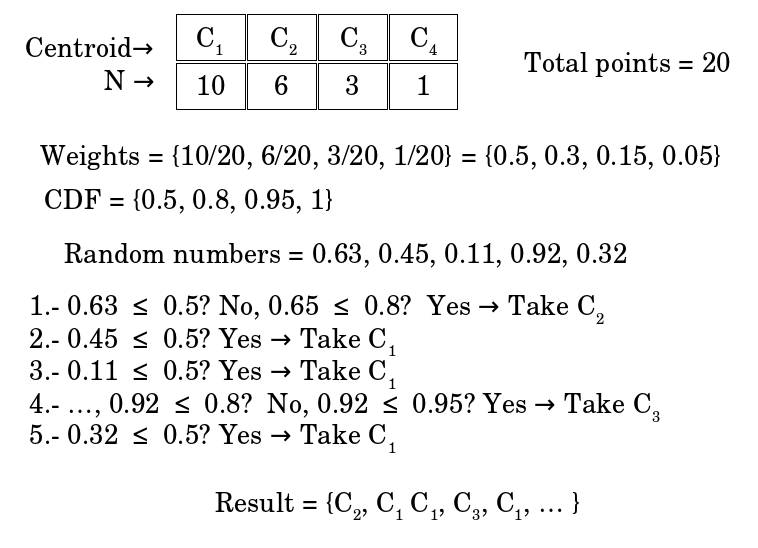
\includegraphics[scale=0.4]{./styles/sampling.png}
 % approxmlast.png: 0x0 pixel, 300dpi, 0.00x0.00 cm, bb=
 \caption{Demonstration: sampling the centroids from weights}
 \label{fig:sampling}
\end{figure}




%-------------------------------------------------------------
\section{Experiments}
\label{sec:experiments}
\subsection{Experiments setting}
For the experiments we used the Network Intrusion dataset~\footnote{Source: http://kdd.ics.uci.edu/databases/kddcup99/kddcup99.html}, which consists of 494,021 instances. For the analysis, we used only the numerical attributes (\#34 out of \#43 attributes).
We vary the speed of the stream and the horizon and we derive two different stream configurations.
The first one, denoted as $DS1$, has a speed $v=2,0000$ points per timestamp and a horizon $H=1$. This implies that the stream lasts for $\frac{494,021}{2,000} \approx 247$ time units. 
The second one, denoted as $DS2$, has a speed of $v=200$ points per timestamp and a horizon $H=256$. Therefore the stream lasts for a period of $\frac{494021}{200} \approx 2470$ time points.

To evaluate the clustering quality, we report in Section~\ref{sec:expQuality} on the sum of squares distance (SSQ) from the points to their nearest micro-cluster, using Euclidean distance as the distance function, within a horizon $H$.

With respect to the efficiency aspect, we report on it in Section~\ref{sec:expScalability}. 

%------------------------------------------------------------------------------------------------------
\subsection{Clustering quality}
\label{sec:expQuality}
We first compare \our to the original \clustream (Section~\ref{sec:expQuality-vs-CluStream}) and then against other stream clustering approaches in Spark (Section~\ref{sec:expQuality-vs-SPARK}).

%------------------------------------------------------------------------------------------------------
\subsubsection{Quality of $Spark-CluStream$ vs original $CluStream$}
\label{sec:expQuality-vs-CluStream}
\paragraph{Results for DS1}
% <<<<<<< HEAD
% We used the same parameters as in~\cite{clustreamOrig}, i.e., $\alpha=2,l=10,InitNumber=2,000,\delta=512,t=2$.
% The parameter $m$, for $m$ last points which is used to estimate the recency of a microcluster, was the only one not provided, we set it to $m=20$. 
$m$ is used to determine the approximate recency value as if the time of arrival of the last $m$ points was averaged.
% For $DS1$, both $m$ and $\delta$ are irrelevant as the threshold is never reached (247 time units vs. 512). 
% The number of micro-clusters was set to $q=50$, which is 10 times the number of final clusters ($5$). 
% =======
The SSQ for $DS1$ is shown in Figure~\ref{fig:DS1quality} for the original $CluStream$ and our $Spark-CluStream$.
We used the same parameters as in~\cite{clustreamOrig}, i.e., $\alpha=2,l=10,InitNumber=2000,\delta=512,t=2$.
The parameter $m$, for $m$ last points, was the only one not provided, we set it to $m=20$. $m$ is used to determine the approximate recency value as if the time of arrival of the last $m$ points was averaged.
For $DS1$, both $m$ and $\delta$ are irrelevant and the reason is that the threshold is never reached (247 time units vs. 512). 
The number of micro-clusters was set to $q=50$, 10 times the number of final clusters ($5$). 
% >>>>>>> b48fee025a90694a4c09982cc46b20463adc1770
% \color{red}@Omar: they suggest 50 and 5 in the original paper?\color{black}\color{blue}@Eirini: yes, they  cluster for k=5  and they recommend 10 times more mcs, they prove that with more than 10 times you don't gain much\color{black}. 
% Also, \textit{fakeKMeans()} used 5,000 sampled points. 
% We report the average results over 4 runs for our \our.

% <<<<<<< HEAD
In Table~\ref{tab:DS1quality} we show the SSQ scores for our \our and the results from \emph{CluStream} as reported in~\cite{CluStream} - these are approximate results ``extracted" from the original paper.
% The SSQ for $DS1$ is shown in Figure~\ref{fig:DS1quality} for the original $CluStream$ and our $Spark-CluStream$.
% For the original $CluStream$ we show the results from the original paper~\cite{clustreamOrig}
%  - in Figure~\ref{fig:2000orig} we also see the performance of the STREAM algorithm, a modified version of $k$-Means for data 
% streams~\cite{STREAM} - the only relevant for the current work is $CluStream$.
% Figure~\ref{fig:2000} shows the results obtained by $Spark-CluStream$. There is a difference in the labels of the horizontal axis; while Figure~\ref{fig:2000orig} shows the time units of the stream, Figure~\ref{fig:2000orig} shows the number of points that had been streamed and processed. The reason is that Spark and the simulated stream  do not deliver the same amount of points for each time unit. %, leading to inaccurate results comparing only by clustering on certain time units. 
% A basic multiplication was used to determine the exact moment in terms of points: $2000\cdot 5 = 10000$, $2000\cdot 20 = 40000$ and so on.
% Comparing the results, it is possible to observe their similarities. We don't know the exact values for Figure~\ref{fig:2000orig} but it suffices to compare the magnitudes of the average SSQ. 
% The exact SSQ scores for $Spark-CluStream$ and the approximated ones from $CluStream$ based on~\cite{CluStream} are shown in Table~\ref{tab:DS1quality}.
Although we don't know the exact values for \emph{CluStream}, we can see that the magnitudes of the average SSQ are comparable.
% =======
% For the original $CluStream$ we show the results from the original paper \cite{clustreamOrig}, as well as the results for \our. Comparing these results, it is possible to observe their similarities. The exact values for \cite{clustreamOrig} are unknown but it suffices to compare the magnitudes of the average SSQ. 
% The exact SSQ scores for $Spark-CluStream$ and the approximated ones from $CluStream$ based on~\cite{clustreamOrig} are shown in Table~\ref{tab:DS1quality}.
% >>>>>>> b48fee025a90694a4c09982cc46b20463adc1770

\begin{table*}[t]
\centering
  \begin{tabular}{|l|l|l|l|l|}\hline
\textbf{$DS1$ - avg SSQ} & \textbf{10k} & \textbf{40k} & \textbf{160k} & \textbf{320k}\\\hline
$CluStream$ & $10^5$-$10^6$ & $10^{12}$-$10^{13}$ & $\approx 10^6$ & $10^2$-$10^3$\\\hline
$Spark-CluStream$ & $3.099\times10^5$ & $6.676\times10^{12}$ & $7.833\times10^5$ & $4.191\times10^2$\\\hline
  \end{tabular}
  \caption{$DS1$ - Average SSQ values}
  \label{tab:DS1quality}
\end{table*}

% <<<<<<< HEAD
% \color{red}@Omar: Can you change the y-axis labels in the second image to match the format of the first? \color{black}
% \color{red}Also, can you change the x-axis label of the second image to "Stream (\#points at clustering time))
% \color{black}\color{blue}DONE\color{black}
% =======
% >>>>>>> b48fee025a90694a4c09982cc46b20463adc1770

%     \begin{figure*}[!ht]
%         \begin{minipage}[l]{1.0\columnwidth}
%             \centering
%              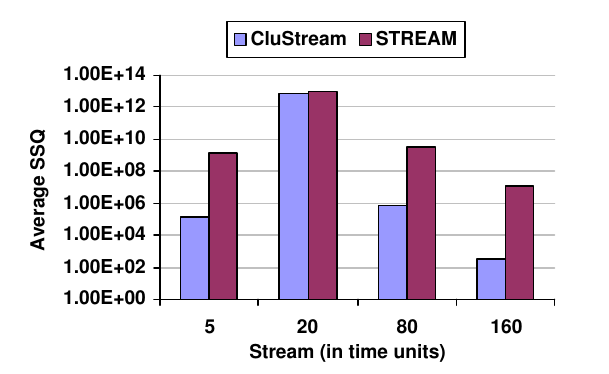
\includegraphics[width=0.9\columnwidth]{./styles/2000h1-orig.png}
%             \caption{SSQ for the original $CluStream$~\cite{clustreamOrig} vs STREAM~\cite{}}\label{fig:2000orig}
%         \end{minipage}
%         \hfill{}
%         \begin{minipage}[r]{1.0\columnwidth}
%             \centering
%             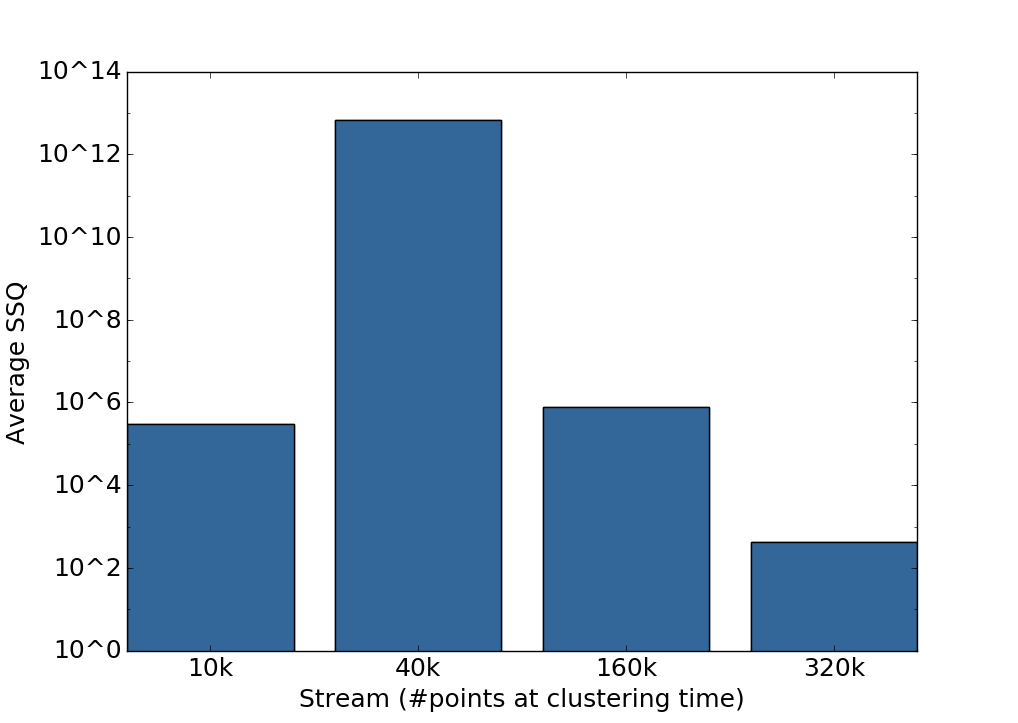
\includegraphics[width=0.9\columnwidth]{./styles/2000h1.png}
%             \caption{SSQ for our $Spark-CluStream$}\label{fig:2000}
%         \end{minipage}
%         \captionsetup{labelformat=empty}
%         \caption{Original $CluStream$ vs SPARK-Clustream.  $DS1$ (Stream speed $v$ = 2,000, $H$=1).}
%         \label{fig:DS1quality}
%     \end{figure*}
    
% Figure \ref{fig:2000orig} shows the results used by the original \textit{CluStream} to show its capabilities against an older method \textit{STREAM}, which is a modified version of K-Means for data streams. The average SSQ for \textit{CluStream} is the most relevant to this test.

% \addtocounter{figure}{-1}
% 
\paragraph{Results for DS2}
% <<<<<<< HEAD
% The SSQ for $DS2$ is shown in Figure~\ref{fig:DS2quality}.
%     \begin{figure*}[!ht]
% =======
% The SSQ for $DS2$ is shown in Figure \ref{fig:DS2quality}.
%  \begin{figure*}[!ht]
>>>>>>> b48fee025a90694a4c09982cc46b20463adc1770
%         \begin{minipage}[l]{1.0\columnwidth}
%             \centering
%              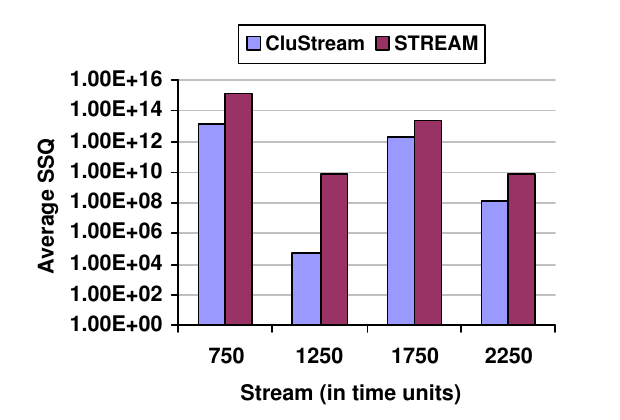
\includegraphics[width=0.9\columnwidth]{./styles/200h256-orig.png}
%             \caption{SSQ for the original $CluStream$~\cite{clustreamOrig} vs STREAM~\cite{}}\label{fig:200h256-orig}
%         \end{minipage}
%         \hfill{}
%         \begin{minipage}[r]{1.0\columnwidth}
%             \centering
%             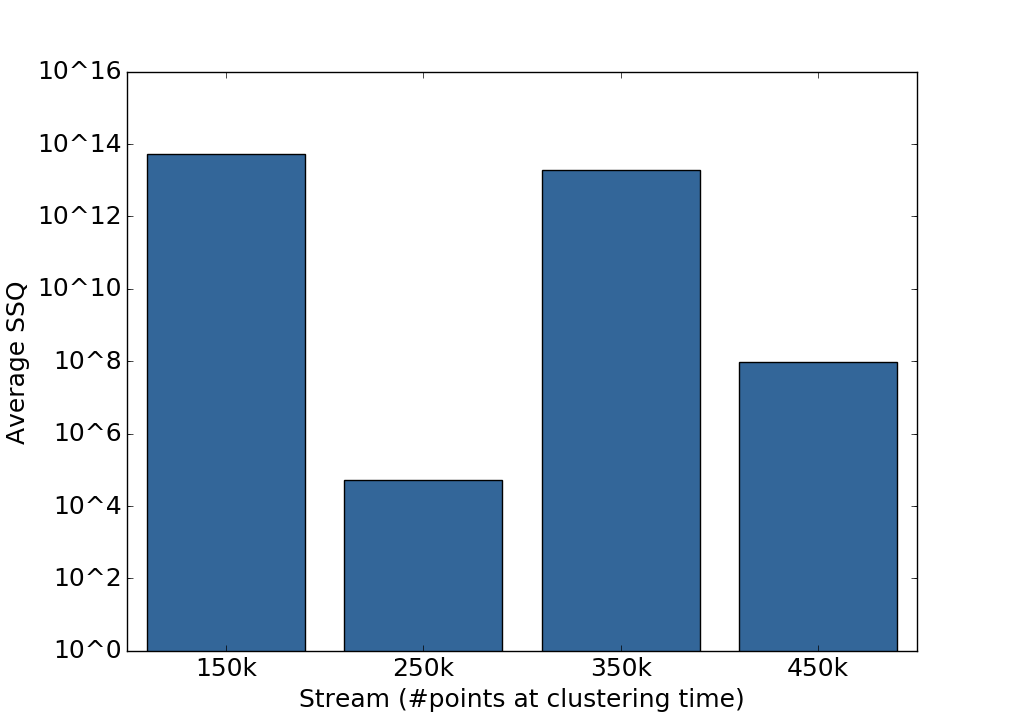
\includegraphics[width=0.9\columnwidth]{./styles/200h256.png}
%             \caption{SSQ for our $Spark-CluStream$}\label{fig:200h256}
%         \end{minipage}
%         \captionsetup{labelformat=empty}
%         \caption{Original $CluStream$ vs SPARK-Clustream. $DS2$ (Stream speed $v$ = 200, $H$=256).}
%         \label{fig:DS2quality}
%     \end{figure*}
% <<<<<<< HEAD
% =======
%     
%  \addtocounter{figure}{-1}
%  
 
% >>>>>>> b48fee025a90694a4c09982cc46b20463adc1770
Parameters were set as for $DS1$.
% The measurement is the SSQ again and the same circumstances apply for this case as in the first one with the difference that here $\delta$ and $m$ are relevant. The parameter $m$ is again chosen to be 20: if 200 points are processed every time unit and there are 50 micro-clusters, assuming all 200 points should be distributed uniformly at least every 5 time units leads to $5\frac{200}{50}=20$. An in-depth analysis of the behavior of \textit{CluStream} for different $\delta$'s and $m$'s is out of the scope of this work. 
% Again, the comparison is for the average SSQ. 
% <<<<<<< HEAD
% The test ran 4 times for \textit{Spark-CluStream} to average the results in both cases, $DS1$ and $DS2$. \color{red} Same for DS1? You run the streams x4 and reported the avg values over the 4 runs?\color{black}\color{blue}Yes, the same process was used\color{black}
The exact scores of \our~and the approximate values from \clustream~are reported %shown in Figure~\ref{fig:DS2quality}; again, they perform similarly. The exact SSQ scores for $Spark-CluStream$ and the approximated ones from $CluStream$ based on~\cite{CluStream} are shown 
in Table~\ref{tab:DS2quality}. Again the quality scores are comparable, i.e., our \our~achieves similar quality clusterings to the original \clustream.
% =======
% The test ran 4 times for \textit{Spark-CluStream} to average the results in both cases, $DS1$ and $DS2$. 
% Again, they perform similarly. The exact SSQ scores for $Spark-CluStream$ and the approximated ones from $CluStream$ based on \cite{clustreamOrig} are shown in Table \ref{tab:DS2quality}.

% >>>>>>> b48fee025a90694a4c09982cc46b20463adc1770
\begin{table*}[t]
\centering
\begin{tabular}{|l|l|l|l|l|}\hline
\textbf{$DS2$ - avg SSQ} & \textbf{150k} & \textbf{250k} & \textbf{350k} & \textbf{450k}\\\hline
CluStream & $10^{13}$-$10^{14}$ & $\approx 10^{5}$ & $10^{12}$-$10^{13}$ & $\approx 10^{8}$\\\hline
Spark-CluStream & $5.402\times10^{13}$ & $5.143\times10^{4}$ & $1.892\times10^{13}$ & $9.646\times10^7$\\\hline
  \end{tabular}
  \caption{$DS2$ - Average SSQ values}
  \label{tab:DS2quality}
\end{table*}

%------------------------------------------------------------------------------------------------------
\subsubsection{$Spark-CluStream$ vs other clustering approaches in SPARK}
\label{sec:expQuality-vs-SPARK}
% <<<<<<< HEAD
We compare our \our against available solutions for stream clustering in Spark and in particular against\textit{Streaming K-Means}~\footnote{More information: https://databricks.com/blog/2015/01/28/introducing-streaming-k-means-in-spark-1-2.html} and\textit{StreamDM-CluStream}~\footnote{More information: http://huawei-noah.github.io/streamDM/}.
% =======
% We compare our \our  against available solutions for stream clustering in Spark and in particular against \textit{Streaming K-Means} and \textit{StreamDM-CluStream}.
% >>>>>>> b48fee025a90694a4c09982cc46b20463adc1770
% , which is another adaptation of \textit{CluStream} for Spark. 
We report here on their clustering quality, the efficiency issue is discussed in Section~\ref{sec:expScalability}.

% We roughly overview these methods hereafter.

% The setup and the dataset are the same as in \ref{validation}, as having already verified results provides the possibility of using those tests to directly compare the results against the other methods. Again, the used measurement is the sum of squares (SSQ).

% Before looking at the results, here are some key considerations for the other methods:

% <<<<<<< HEAD
% \begin{itemize}%  \item \textit{Streaming K-Means~\footnote{More information: https://databricks.com/blog/2015/01/28/introducing-streaming-k-means-in-spark-1-2.html}}:
%  \begin{itemize}
%   \item In order to have comparable results, the time horizon $H$ must be interpreted differently. There are two strategies: the first option is to use the parameter \textit{halfLife}, which can be configured to let the algorithm to completely adjust the clusters after $HL$ points or batches.
%   \item The alternative would be to set the $decayFactor$, which sets the weight for the clusters of the "old" data (only the current batch is considered "new" data). This is a number between 0 and 1, such that if it is 0 then only the clusters for "new" data determine the final clusters, if it is set to 1, then the clusters of past data will have the same influence on the final clusters. It is important to notice that this \textit{decayFactor} also considers the number of points of the "new" and "old" data, so in the last case, after a long time, "new" data will have little influence as the number of points of the current batch will be considerable smaller than the points clustered so far.
%  \end{itemize}
%  \item \textit{StreamDM-CluStream~\footnote{More information: http://huawei-noah.github.io/streamDM/}}:
%  \begin{itemize}
%   \item This adaptation of \textit{CluStream} does not include the offline part as a separate module, meaning that it does not save snapshots and therefore it has to perform the macro-clustering process for every batch. This brings some limitations, the horizon $H$ no longer has the same meaning: the $\delta$ parameter is used instead as an equivalent, relying on the micro-clustering part only and its ability to delete and create new micro-clusters.
% \end{itemize}
% \end{itemize}
% \color{black}
% =======
% \begin{itemize}
%  \item \textit{Streaming K-Means~\footnote{More information: https://databricks.com/blog/2015/01/28/introducing-streaming-k-means-in-spark-1-2.html}}:
%  \begin{itemize}
%   \item In order to have comparable results, the time horizon $H$ must be interpreted differently. There are two strategies: the first option is to use the parameter \textit{halfLife}, which can be configured to let the algorithm to completely adjust the clusters after $HL$ points or batches.
%   \item The alternative would be to set the $decayFactor$, which sets the weight for the clusters of the "old" data (only the current batch is considered "new" data) to calculate the new centroids.
%  \end{itemize}
%  \item \textit{StreamDM-CluStream~\footnote{More information: http://huawei-noah.github.io/streamDM/}}:
%  \begin{itemize}
%   \item This adaptation of \textit{CluStream} does not include the offline part as a separate module, meaning that it does not save snapshots and therefore it has to perform the macro-clustering process for every batch. This brings some limitations, the horizon $H$ no longer has the same meaning: the $\delta$ parameter is used instead as an equivalent, relying on the micro-clustering part only and its ability to delete and create new micro-clusters.
% \end{itemize}
% \end{itemize}
% >>>>>>> b48fee025a90694a4c09982cc46b20463adc1770

\paragraph{Results on $DS1$}
For the $DS1$ stream the results are shown in Figure~\ref{fig:comparison2000}. %The number of clusters $k$ is always 5 for this dataset in all the experiments.
For \textit{Streaming K-Means}, the horizon $H=1$ is transformed to $halfLife=1,000$ points, as the stream speed is 2,000 points. %This is because the speed of the stream is 2,000 points per time unit, if the horizon is 1, then only 2000 points are desired to be clustered, and half of that results in 1000 points. 
The \textit{decayFactor} is set to 0, i.e., only the last 2,000 points will influence on the clusters. %, which is exactly what is desired.
\textit{StreamDM-CluStream} is set up with its default parameters, only changing the horizon to 1 and the number of micro-clusters to 50 to match those of \our.
%
\begin{figure}[h]
 \centering
 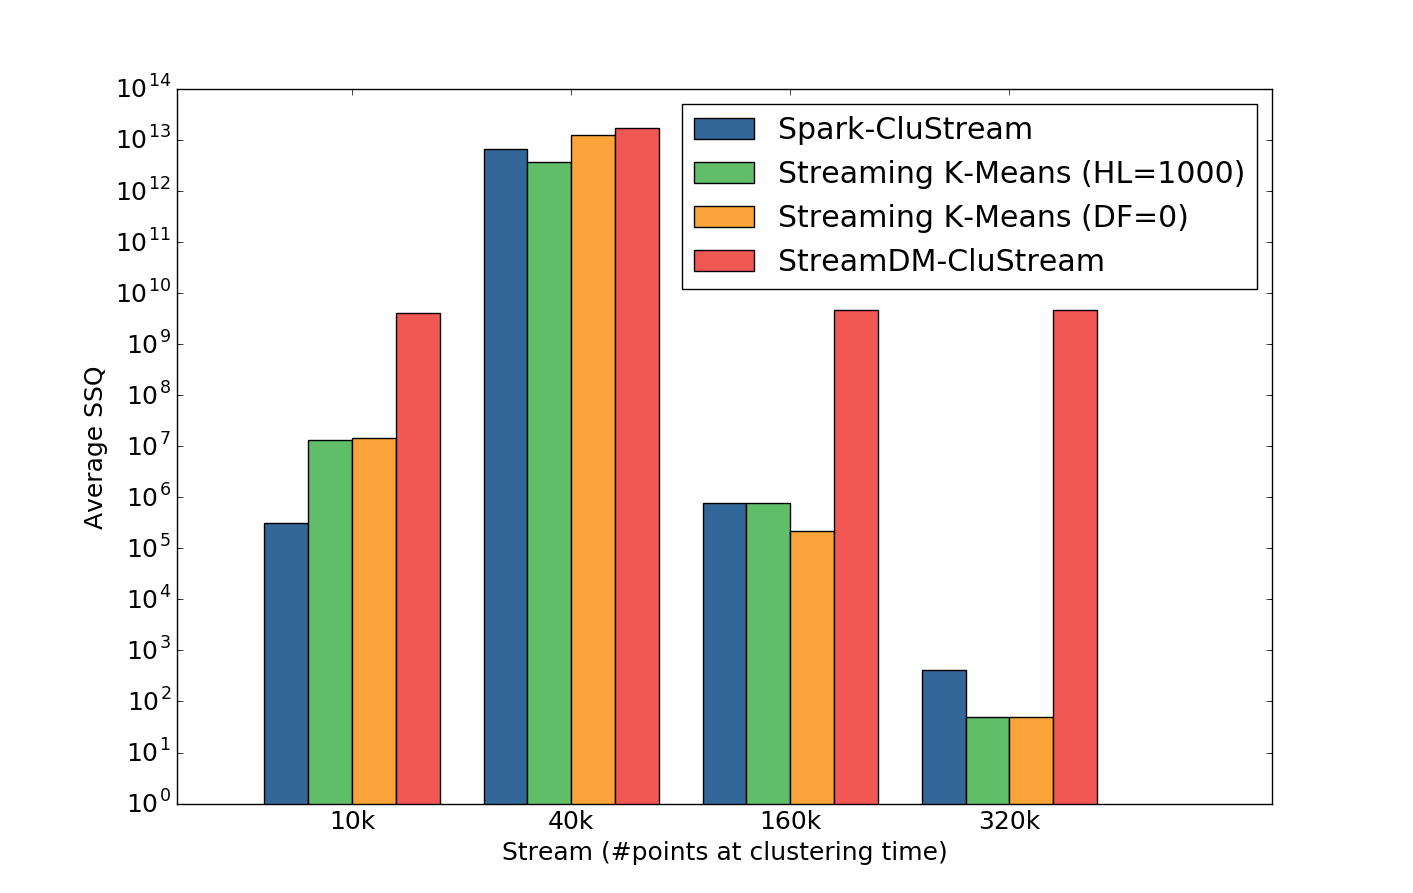
\includegraphics[scale=0.265]{./styles/comparison2000.png}
 \caption{Average SSQ for different stream clustering methods in SPARK. $DS1$ (Stream speed $v$ = 2,000, $H$=1)}
 \label{fig:comparison2000}
\end{figure}
% <<<<<<< HEAD
%
As we can see, our \our~delivers results which are very close to those of \textit{Streaming K-Means}, whereas \textit{Streaming K-Means} with the \textit{decayFactor} (DF) is the best.
% expected to do well on this test as it could be configured to cluster exactly as it was intended for this dataset. 
The surprising results come from \textit{StreamDM-CluStream}, which is the worse among the tested methods, especially for the last two points, i.e., at $160k$ and $320k$.
% To understand this behavior, we performed another experiment with \our~without snapshots. For both methods we used a horizon $H = 1$ and $m=100$. 
% \color{red}@Omar: what is m?\color{black}\color{blue}UPDATED THE EXPLANATION ABOVE \color{black}.
To further investigate this, we conduct another experiment where we compare \our~without snapshots against \textit{StreamDM-CluStream}. The results are shown in Figure \ref{fig:comparisonNoSnaps}.
% =======

% From Figure~\ref{fig:comparison2000} it can be seen that our \our~delivers results which are very close to those of \textit{Streaming K-Means}. Also, \textit{Streaming K-Means} with the \textit{decayFactor} (DF) is expected to do well on this test as it could be configured to cluster exactly as it was intended for this dataset. 
% The surprising results come from \textit{StreamDM-CluStream}, as it performs worse than the rest of the methods, especially for the last two points, i.e.,  at $160k$ and $320k$.
% To understand this behavior, we performed another experiment with \our~without snapshots. For both methods we used a horizon $H = 1$ and $m=100$.
% >>>>>>> b48fee025a90694a4c09982cc46b20463adc1770
\begin{figure}[h]
 \centering
 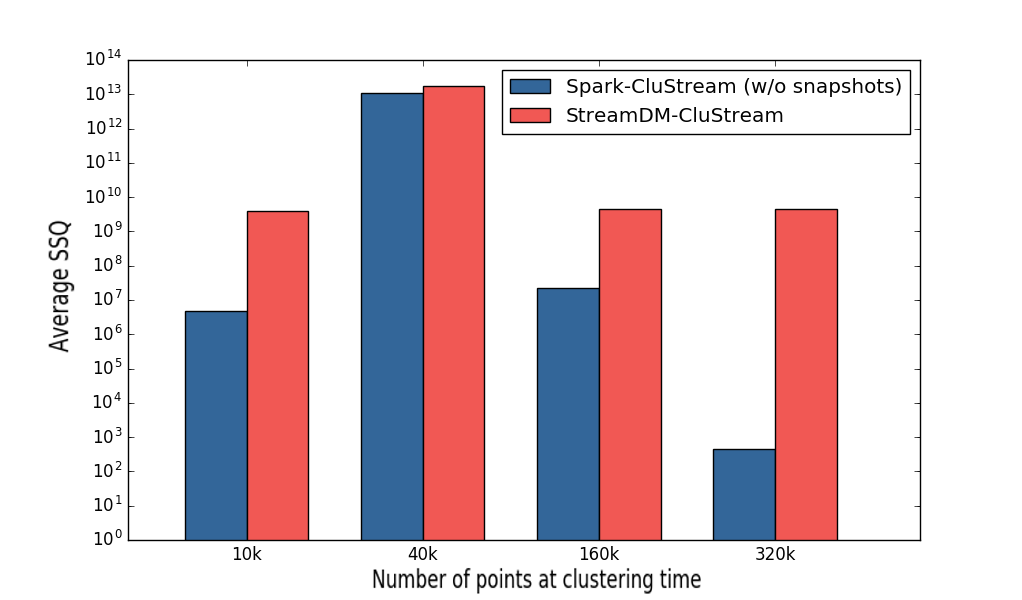
\includegraphics[scale=0.24]{./styles/comparisonNoSnaps.png}
 \caption{\our without snapshots vs \textit{StreamDM-CluStream}. $DS1$ (Stream speed $v=2,000$, $H=1$, $m=100$).}
 \label{fig:comparisonNoSnaps}
\end{figure}
As we can see, \our outperforms \textit{StreamDM-CluStream} even if we remove the snapshot part, but the quality is lower comparing to the snapshot version.
%  shows poorer results for \textit{Spark-CluStream} in comparison to its original behavior with snapshots, but still delivers noticeably better results than \textit{StreamDM-CluStream}, even though all these tests were executed 4 times and the SSQ erros were averaged to get a better representation of how these methods perform.

%-------------------------------------
\paragraph{Results on $DS2$}
% <<<<<<< HEAD
For the $DS2$ stream the results are shown in Figure~\ref{fig:comparison200}.
% Repeating the experiment for the stream with a speed of 200 and a horizon $H=256$ revealed unexpected results. 
All parameters remained the same for all methods, except for the $halfLife$ parameter for \textit{Streaming K-Means}, which is set to  $halfLife=25,600$ ($200\cdot 256=51,200$).
% We computer the new $halfLife$ as follows: multiplying the speed of the stream to the horizon, $200\cdot 256=51200$ shows how many points of the stream are supposed to be clustered at each time, indicating that the parameter should be set to $halfLife=25,600$. 
We calculate the $decayFactor$ as follows: 
% The \textit{decayFactor} strategy at first seems that does not work for such an experiment, but considering that the total number of entries and the exact clustering points are known, it is possible to calculate an average value to use as a $decayFactor$:  
% \begin{itemize}
%  \item 
At 150,000 points, the ratio of the points to cluster to the total number of points at that particular time is $\frac{51,200}{150,000} \approx 0.3413$.
%  \item 
At 250,000 points, this equals to $\frac{51,200}{250,000} \approx 0.2048$.
%  \item 
At 350,000 points, this equals to $\frac{51,200}{350,000} \approx 0.1462$.
%  \item 
At 450,000 points, this equals to $\frac{51,200}{450,000} \approx 0.1137$.
% \end{itemize}
Averaging those ratios leads to a \textit{decayFactor = 0.2015}. %, which is a way to determine how important the old data is in comparison to the new one.
\begin{figure}[h!]
 \centering
 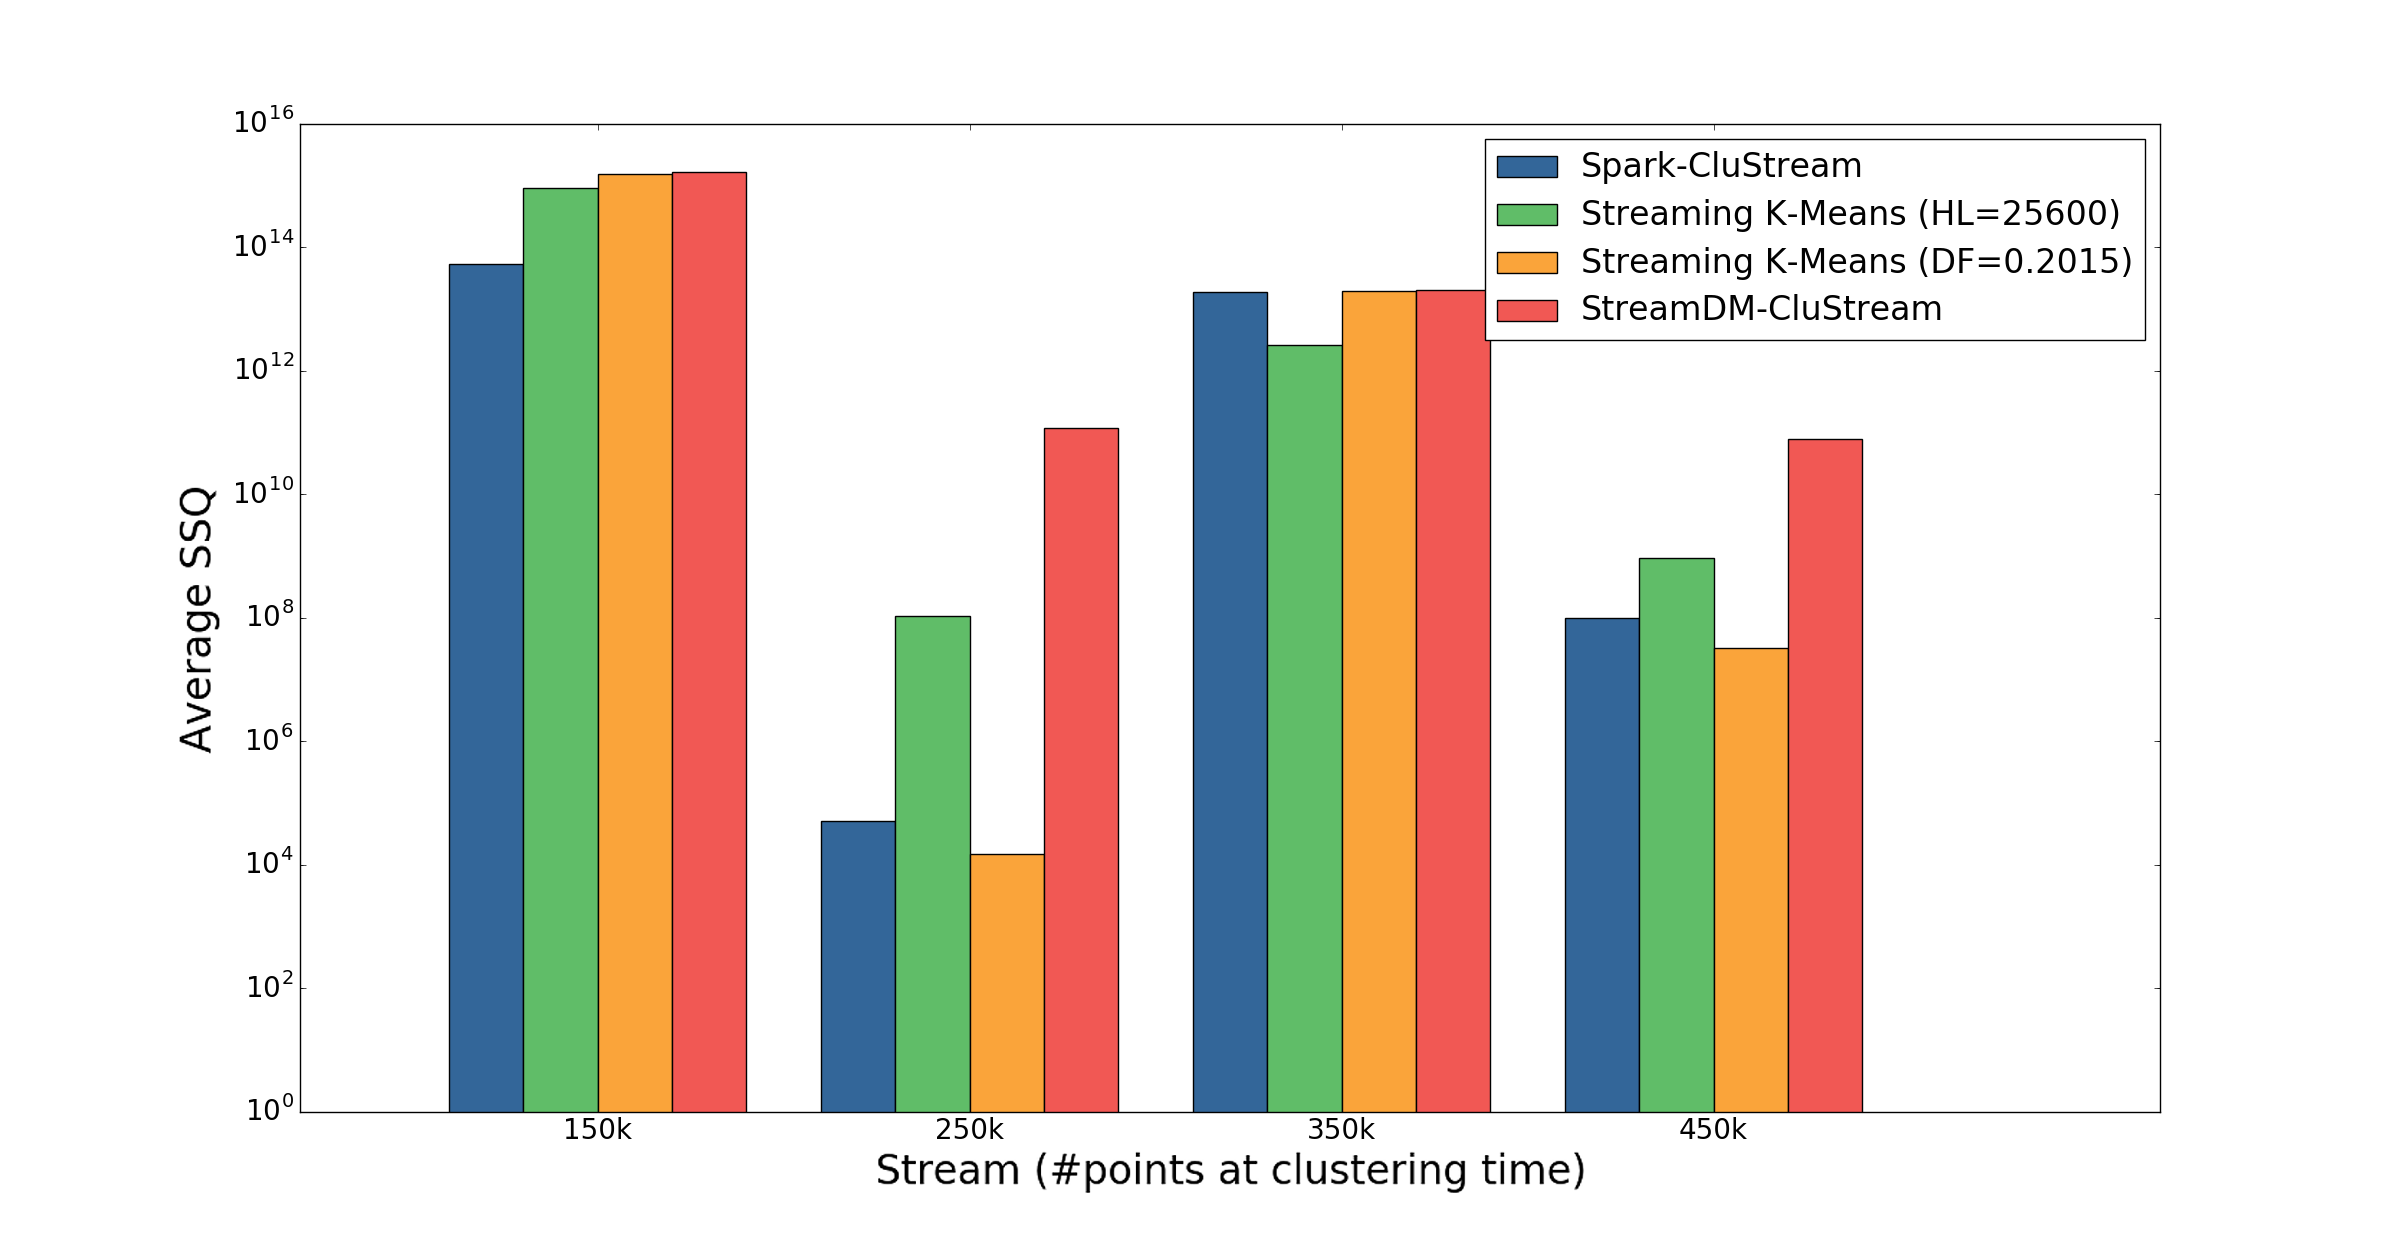
\includegraphics[scale=0.15]{./styles/comparison200.png}
%  \caption{Comparison results: all methods. Stream speed = 200, H=256}
 \caption{Average SSQ for different stream clustering methods in SPARK. $DS2$ (Stream speed $v$ = 200, $H$=256)}
 \label{fig:comparison200}
\end{figure}
As we can see, \our performs consistently well and better than \textit{StreamDM-CluStream}. As expected \textit{Streaming K-Means} with the \textit{decayFactor} achieves the best performance.

We repeat the without-snapshot experiment, the results are shown in Figure \ref{fig:comparisonNoSnaps2}.
\begin{figure}[h]
 \centering
 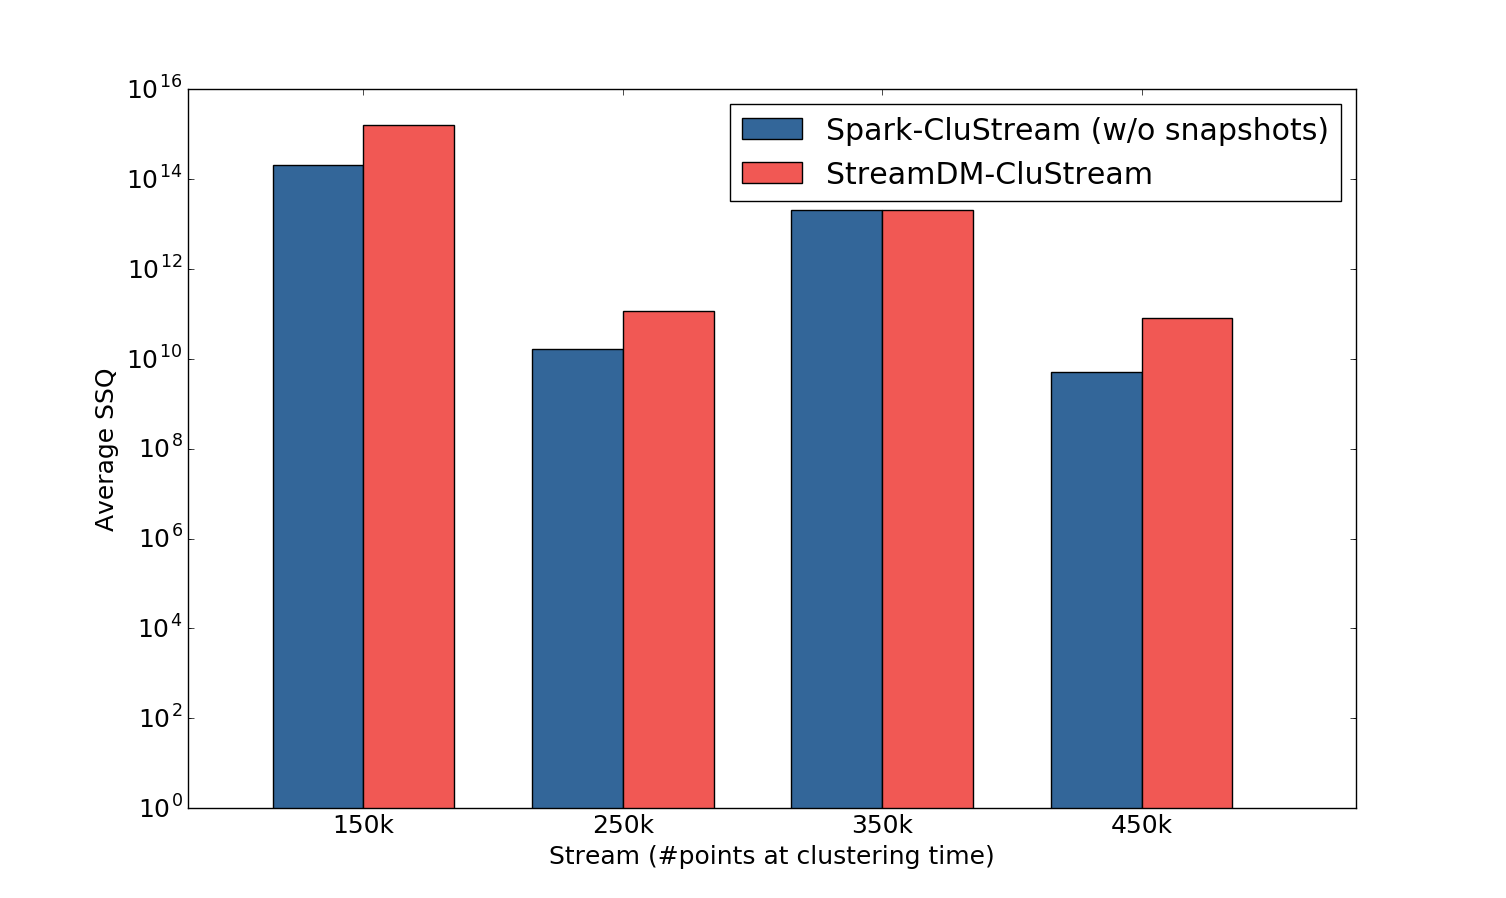
\includegraphics[scale=0.24]{./styles/comparisonNoSnaps2.png}
  \caption{\our without snapshots vs \textit{StreamDM-CluStream}. $DS2$ (Stream speed $v=200$, $H=256$, $m=100$).}
 \label{fig:comparisonNoSnaps2}
\end{figure}
As we can see, \our~delivers better results than \textit{StreamDM-CluStream} but the difference is reduced significantly comparing to $DS1$. These results might indicate that \textit{StreamDM-CluStream}  benefits from larger horizons.
% =======
% For the $DS2$ stream the results are shown in Figure~\ref{fig:comparison2000}.

% Repeating the experiment for the stream with a speed of 200 and a horizon $H=256$ revealed unexpected results. While most parameters for all methods remained the same, for \textit{Streaming K-Means} a new $halfLife$ has to be calculated: multiplying the speed of the stream to the horizon, $200\cdot 256=51200$ shows how many points of the stream are supposed to be clustered at each time, indicating that the parameter should be set to $halfLife=25600$. 


% The \textit{decayFactor} strategy at first seems that does not work for such experiment, but considering that the total number of entries is known and exactly the marks at which the clustering process happens, it is possible to calculate an average value to use as a $decayFactor$: 

% \begin{itemize}
%  \item At 150000 points: $\frac{51200}{150000} \approx 0.3413$, which is the ratio of the points to cluster to the total number of points at that particular time.
%  \item At 150000 points: $\frac{51200}{250000} \approx 0.2048$.
%  \item At 150000 points: $\frac{51200}{350000} \approx 0.1462$.
%  \item At 150000 points: $\frac{51200}{450000} \approx 0.1137$.
% \end{itemize}

% Averaging those ratios leads to a \textit{decayFactor = 0.2015}, which is a way to determine how important the old data is in comparison to the new one.

% \begin{figure}[h!]
%  \centering
%  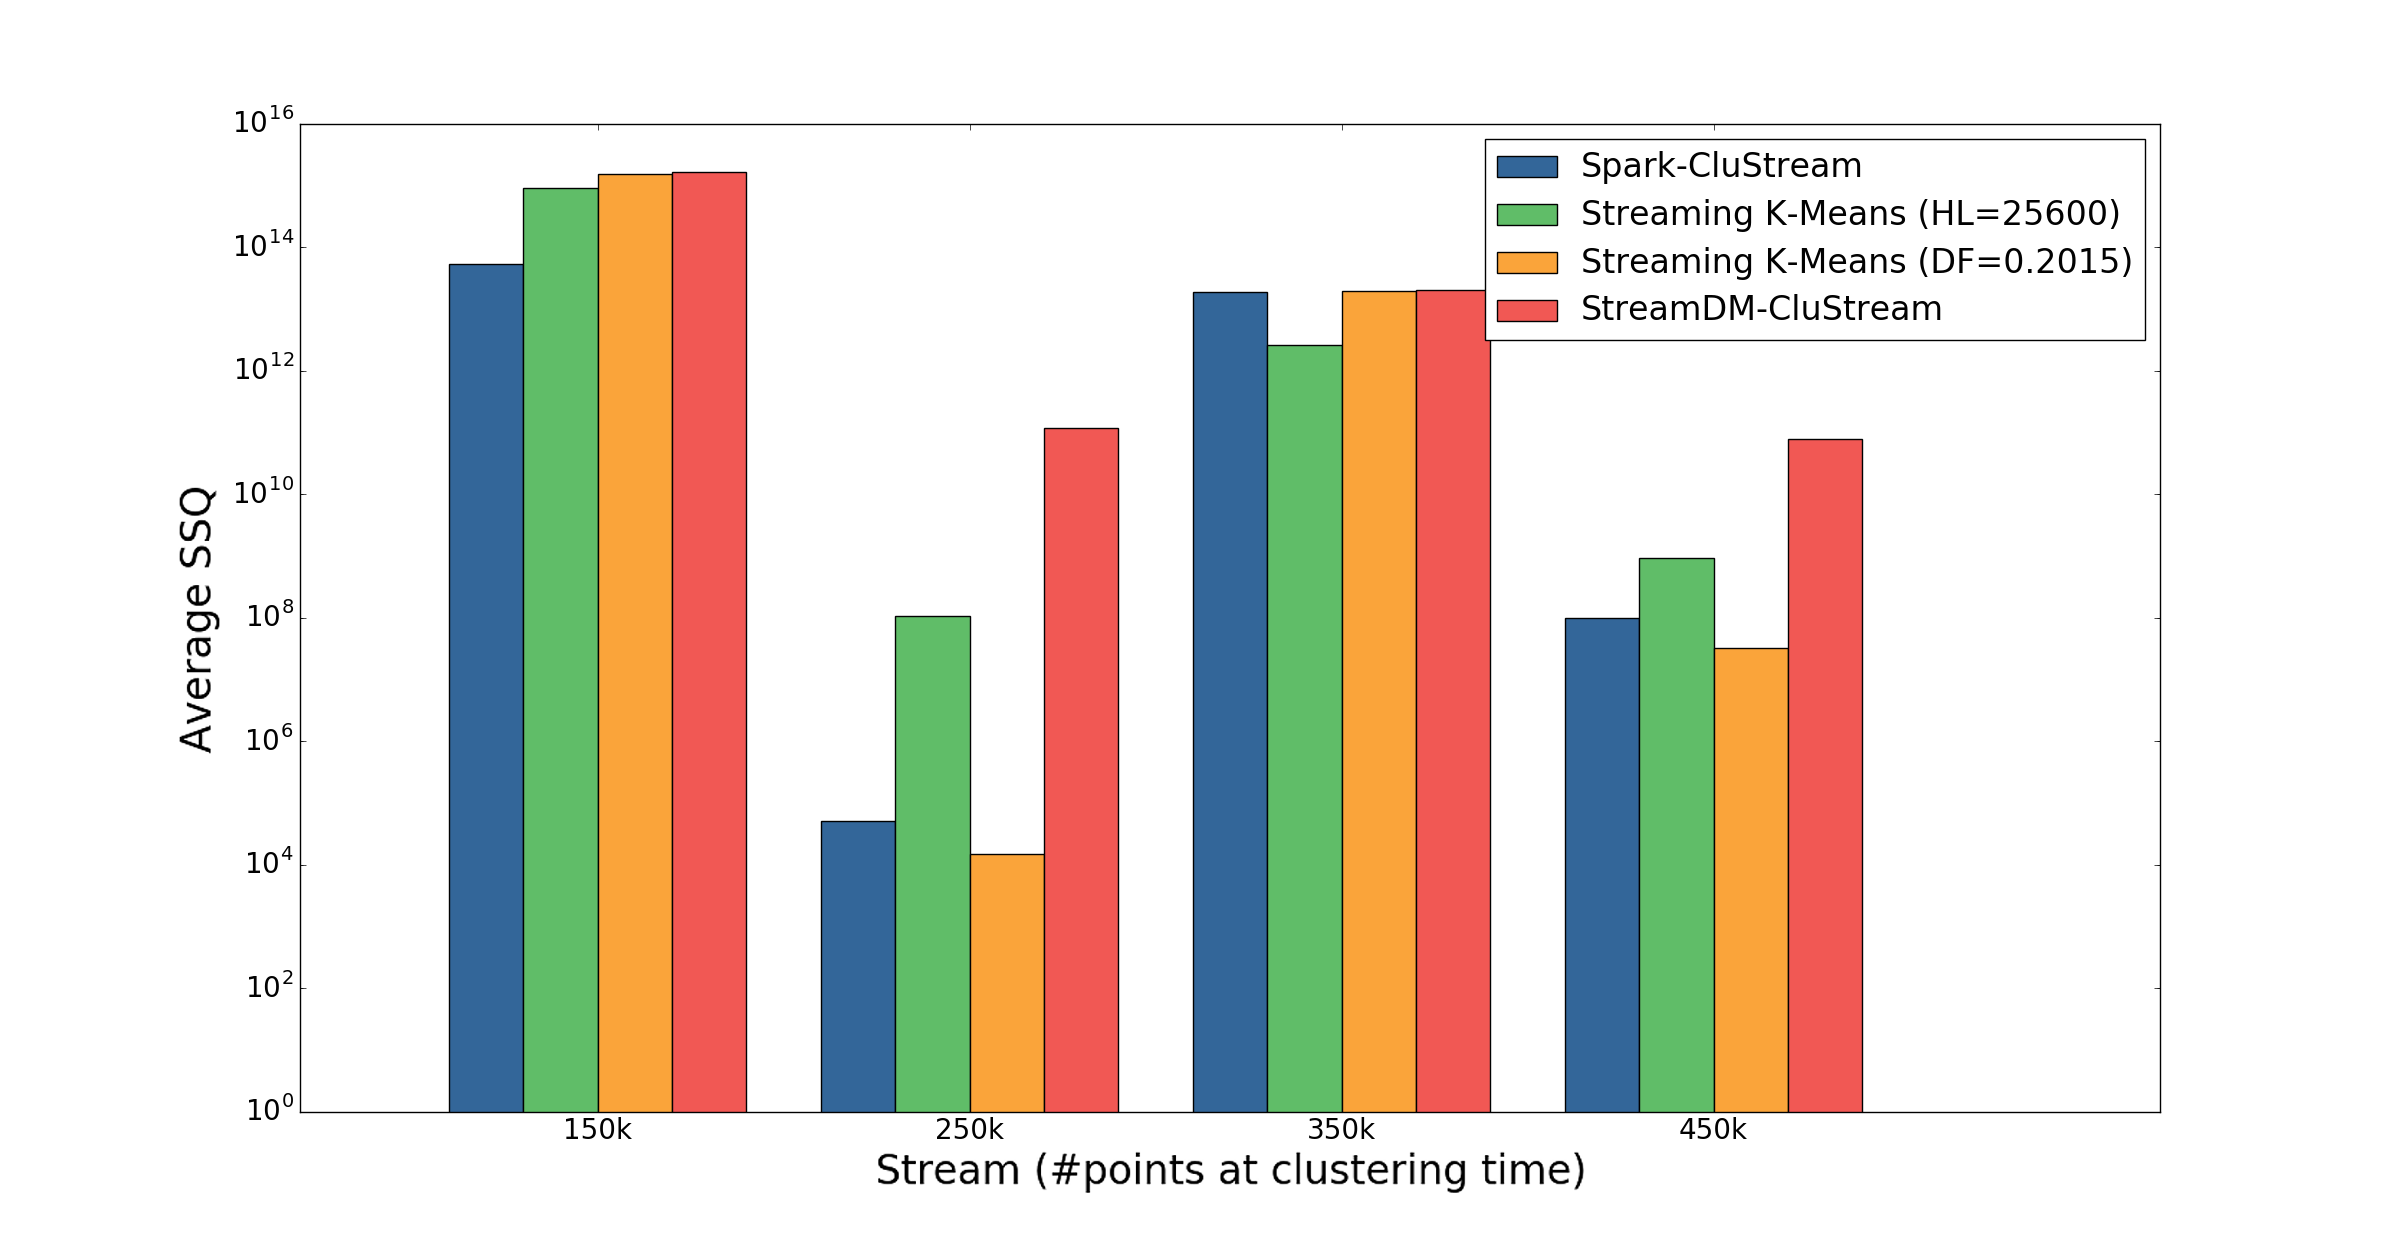
\includegraphics[scale=0.16]{./styles/comparison200.png}
%  \caption{Comparison results: all methods. Stream speed = 200, H=256}
%  \label{fig:comparison200}
% \end{figure}

% Figure \ref{fig:comparison200} shows that while \textit{Spark-CluStream} still performs consistently good, \textit{Streaming K-Means} with the \textit{decayFactor} outperformed its relative with the $halfLife$ strategy. Another thing to notice is that \textit{StreamDM-CluStream} still delivered the worse results. 


% >>>>>>> b48fee025a90694a4c09982cc46b20463adc1770



%------------------------------------------------------------------------------------------------------
\subsection{Scalability}
\label{sec:expScalability}
We test the scalability with respect to data dimensionality and number of microclusters, using data generated by a \textit{Random Radial Basis Function} generator.

The scalability tests are performed in two different scenarios: one being an analysis of how it scales for different number of attributes (dimensions of the data points) using only 20 micro-clusters and the other one using 200 micro-clusters. The reason behind this is that the number of attributes and the number of final clusters for a specific purpose are two key factors which determine the complexity of \textit{Spark-CluStream}. The speed of the stream is controlled for 10000 points for every batch of data because it is easier to test the scalability when many computations have to be done.

Any application using Spark streaming assigns one core exclusively to handle the stream, therefore the minimum number of processors required is two, this also means that using 2 processors is equivalent to using a single processor to execute the application. The number of processors mentioned in these tests is the total, but the real number of processors used for the computations is that number minus one.


\begin{figure*}[!ht]
        \begin{minipage}[l]{1.0\columnwidth}
            \centering
             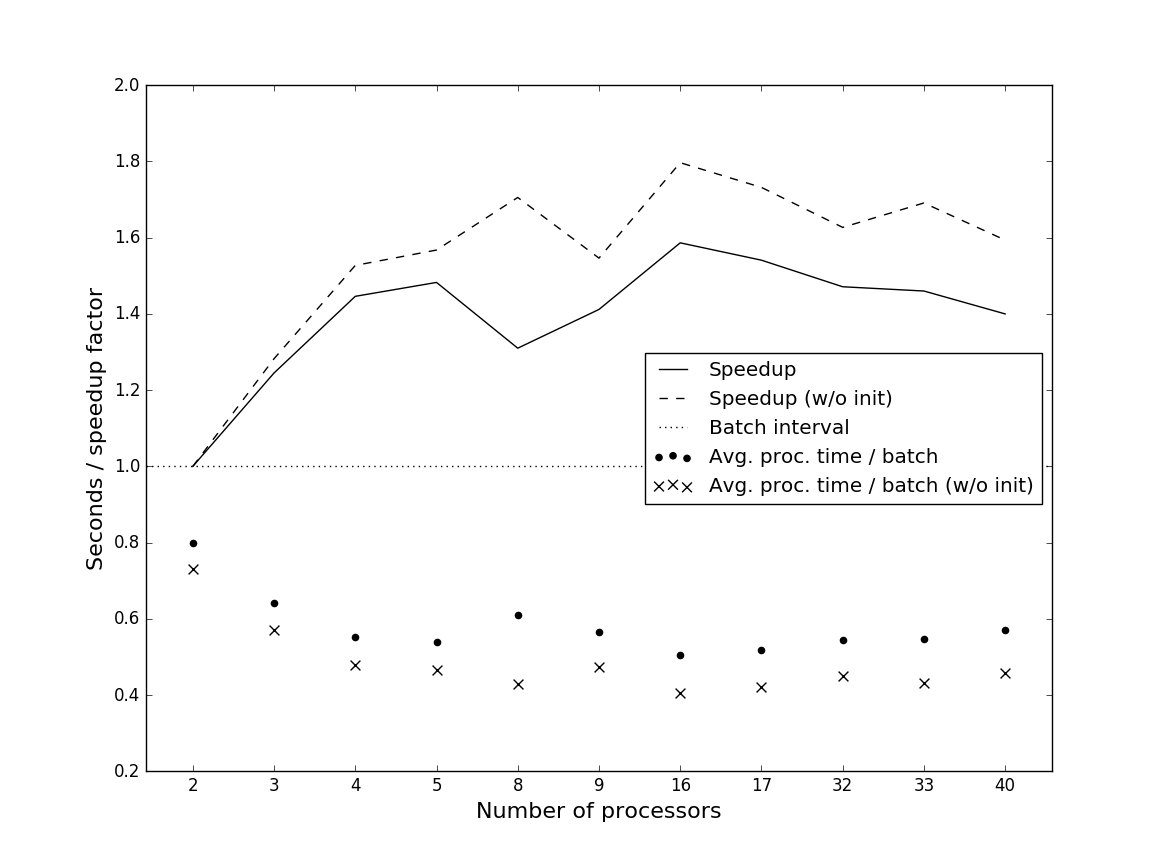
\includegraphics[width=0.9\columnwidth]{./styles/perf20-2.png}
            \caption{Dimension: $d$ = 2}
            \label{fig:perf20-2}
        \end{minipage}
        \hfill{}
        \begin{minipage}[r]{1.0\columnwidth}
            \centering
            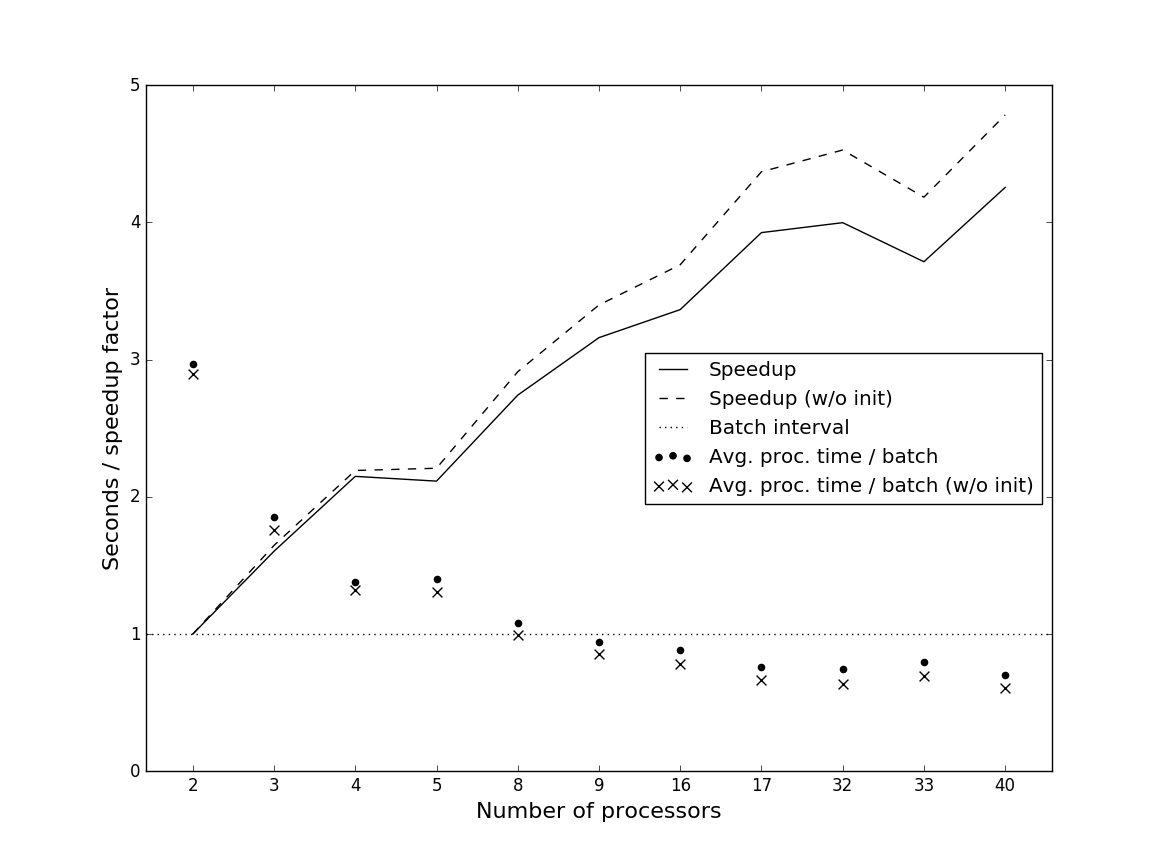
\includegraphics[width=0.9\columnwidth]{./styles/perf20-100.png}
            \caption{Dimension: $d$ = 100}\label{fig:perf20-100}
        \end{minipage}
        \captionsetup{labelformat=empty}
	\caption{Scalability-dimensionality comparison for Stream speed = 10000 and q = 20}
	 \label{fig:DS1quality}
\end{figure*}
\addtocounter{figure}{-1}
The charts here presented show the speedup obtained by increasing the number of processors from 2 to 40, which in reality means that 1 to 39 processors where used for the computations. It also shows the average processing time for each batch of data. Because the initialization takes the most amount of time, it is also convenient to show these values without considering that process: by doing so it is possible to see what would be the expected results for a longer run, where the initialization is no longer dominant. Finally it shows the interval time for which Spark process a new batch of data, in particular all these tests processed batch every second.


Figure \ref{fig:perf20-2} shows that using only 20 micro-clusters and 2 dimensions has poor scalability, not even being able to perform twice as fast as for a single processor (2 in total). Even for this high speed streaming, one processor is enough to process the batches of data before a new batch is processed, meaning that the setup is stable.

\begin{figure*}[!ht]
        \begin{minipage}[l]{1.0\columnwidth}
            \centering
             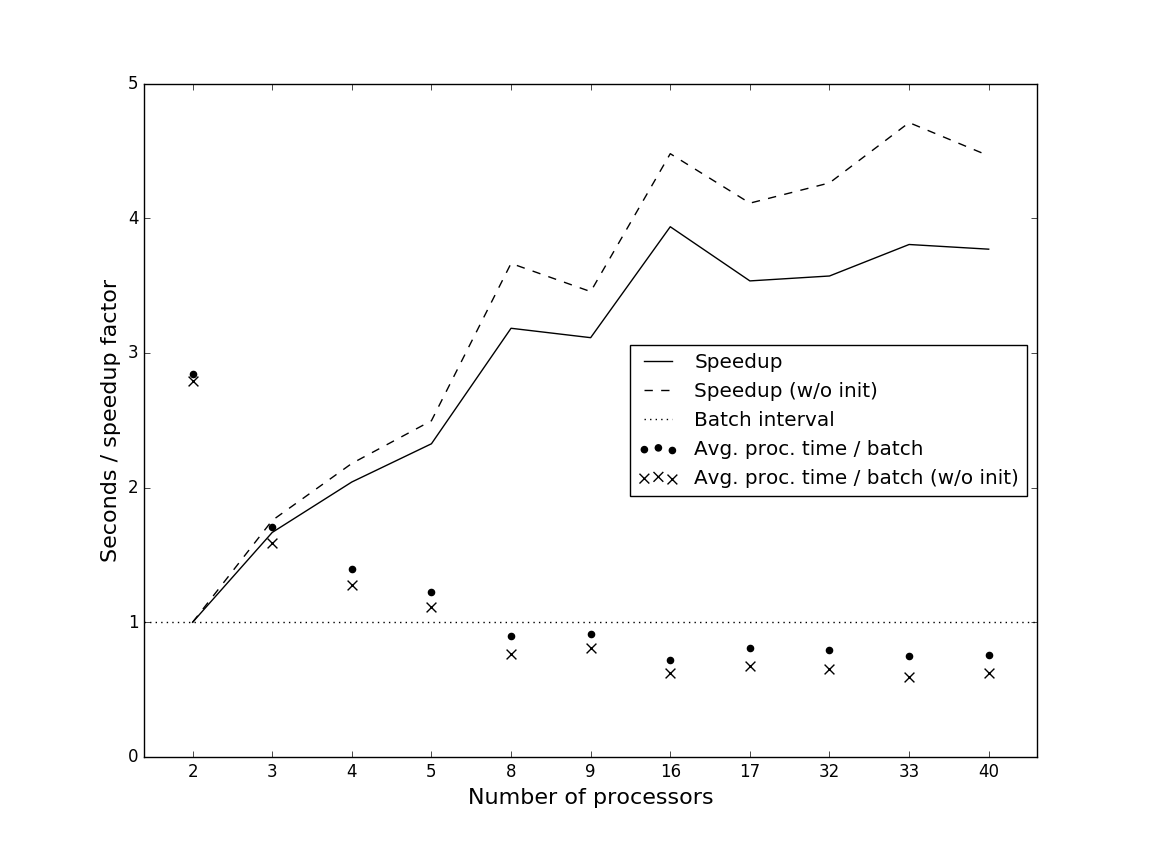
\includegraphics[width=0.9\columnwidth]{./styles/perf200-2.png}
            \caption{Dimension: $d$ = 2}
            \label{fig:perf200-2}
        \end{minipage}
        \hfill{}
        \begin{minipage}[r]{1.0\columnwidth}
            \centering
            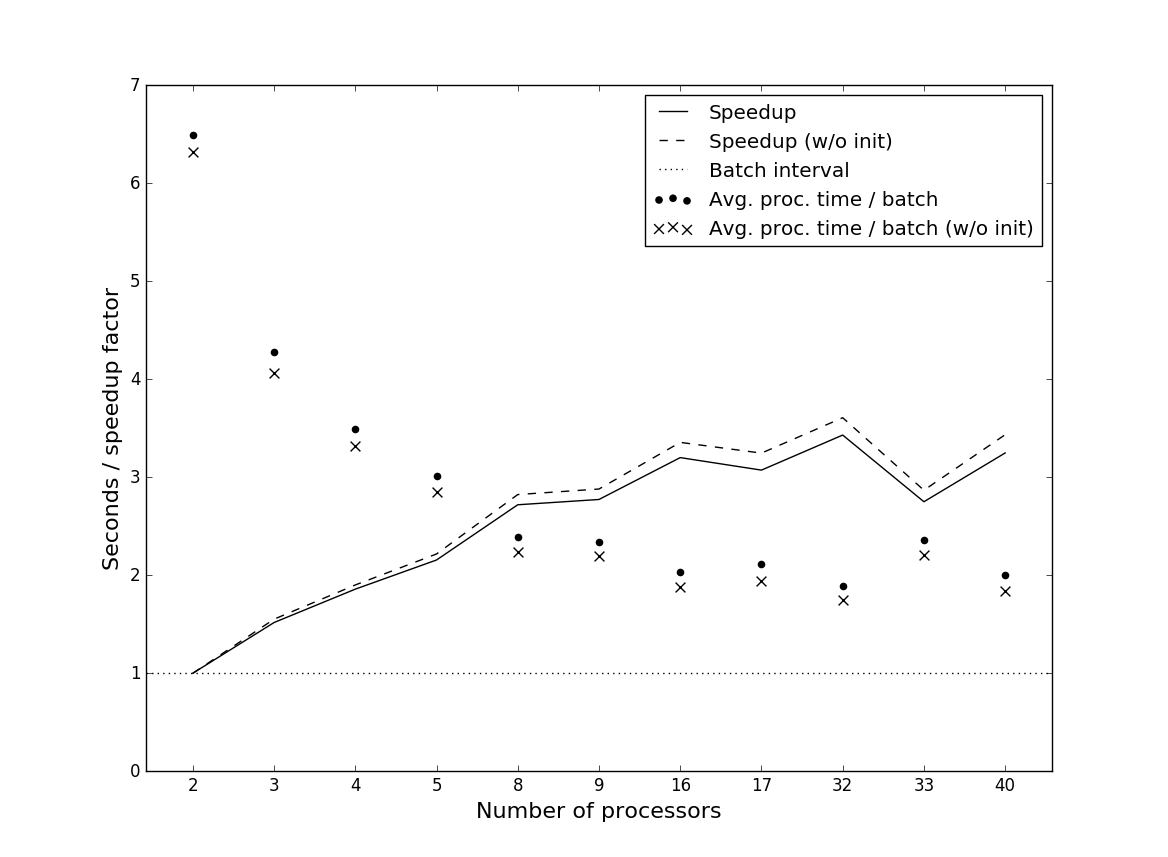
\includegraphics[width=0.9\columnwidth]{./styles/perf200-100.png}
            \caption{Dimension: $d$ = 100}\label{fig:perf200-100}
        \end{minipage}
        \captionsetup{labelformat=empty}     
        \caption{Scalability-dimensionality comparison for Stream speed = 10000 and q = 200}
        \label{fig:DS2quality}
\end{figure*}

\addtocounter{figure}{-1}
Increasing the dimensionality of the points increases the computational effort needed to process the points in every batch of data and here is where \textit{Spark-CluStream} shows its scalability, which is almost linear\footnote{By linear scalability does not mean it scales with a 1 to 1 ratio, but rather linearly proportional.} for up to 16-17 processors, as it can be seen in Figure \ref{fig:perf20-100}.  From the average processing time per batch, it can be seen that from 32 to 40 processors it does not improve much anymore and the speedup does not increase quasi-linearly anymore. Here a total of 9 processors were required to stabilize \textit{Spark-CluStream}. 


Interestingly, increasing the number of micro-clusters by a factor of 10 for 2 attributes resulted in good scalability, similarly to the scenario with 20 micro-clusters and 100 attributes. Here a total of 8 processors were enough for a stable run, as shown in Figure \ref{fig:perf200-2}.



Finally, when the number of clusters and the number of attributes are both increased significantly, Figure \ref{fig:perf200-100} shows for \textit{Spark-CluStream} quasi-linear scalability but this time only up to about 8-9 processors. After that point, the speedup slows down showing almost no improvement after 16 processors. This test never reached a stable configuration.


\subsection{Performance}

In this section, the scalability of \textit{Spark-CluStream} is compared to that of \textit{StreamDM-CluStream} and Spark's \textit{Streaming K-Means} unsing the Spark cluster setup for $q=20$ and $d=2,100$, for the $CluStream$ method. Also, a test on a signle machine is performed.


\begin{figure}[h!]
 \centering
 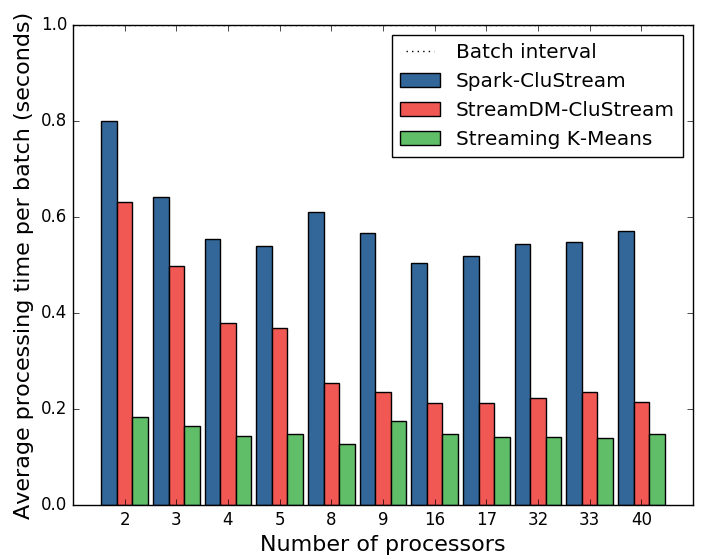
\includegraphics[scale=0.45]{./styles/perfComp2.png}
 \caption{Processing time comparison: $q=20$, $d=2$}
 \label{fig:perfComp2}
\end{figure}

In Figure \ref{fig:perfComp2} it can be seen that \textit{Spark-CluStream} took the most time on average to process a batch of data and being \textit{Streaming K-Means} the fastets among the three. 

\begin{figure}[h!]
 \centering
 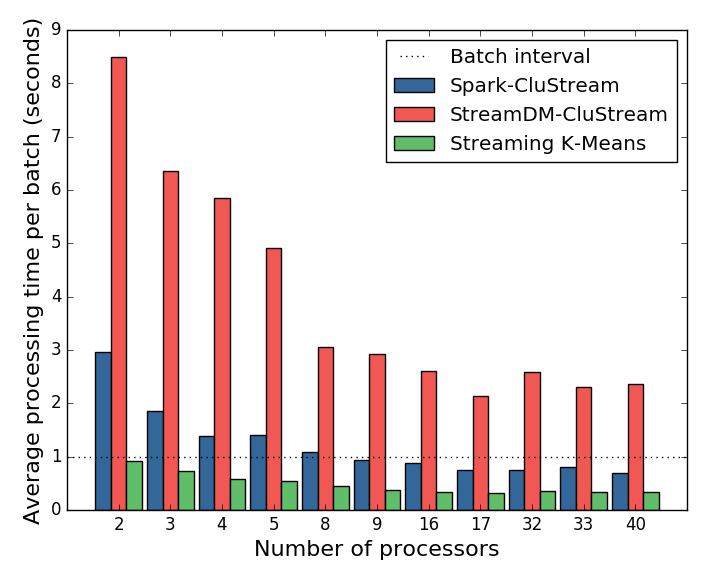
\includegraphics[scale=0.45]{./styles/perfComp100.png}
 \caption{Processing time comparison: $q=20$, $d=100$}
 \label{fig:perfComp100}
\end{figure}

When it comes to higher dimensions, \textit{Spark-CluStream} shows a significant improvement over \textit{StreamDM-CluStream}, which never got to the point were it was stable (below the 1 second mark), as shown in \ref{fig:perfComp100}, it seems to scale as fast as \textit{Spark-CluStream} but it was not enough even with 40 processors. 


\begin{figure}[h!]
 \centering
 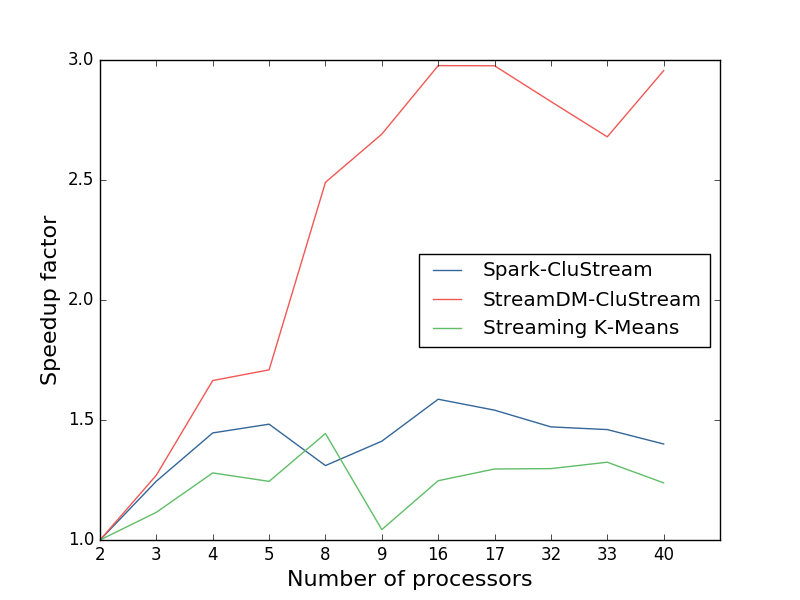
\includegraphics[scale=0.45]{./styles/scalComp2.png}
 \caption{Scalability comparison: $q=20$, $d=2$}
 \label{fig:scalComp2}
\end{figure}

Surprisingly, in Figure \ref{fig:scalComp2}, \textit{StreamDM-CluStream} shows to be able to scale even for this tests, while both \textit{Spark-CluStream} and \textit{Streaming K-Means} seem to struggle taking advantage of using more processors.

\begin{figure}[h!]
 \centering
 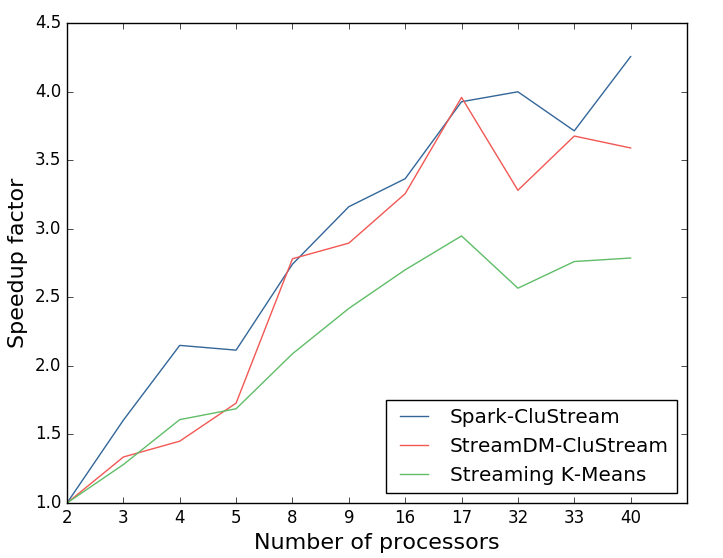
\includegraphics[scale=0.45]{./styles/scalComp100.png}
 \caption{Processing time comparison: $q=20$, $d=100$}
 \label{fig:scalComp100}
\end{figure}

Figure \ref{fig:scalComp100} shows that all three algorithms are able to scale similarly for this test, being \textit{Spark-CluStream} the one having a very slight advantage as it does not slow down as quickly as the other two.



Another interesting comparison, is the processing time per batch of data for a single machine, using a real dataset such as the \textit{Network Intrusion}. Here, communication is less of an issue as all the partitions lie in the same share memory space, and still there are 4 virtual cores in disposition for the algorithms to run. 

The test was performed using a stream speed of 2000 points per batch and with a horizon $H=1$, to match one of the validation tests.

\begin{figure}[h!]
 \centering
 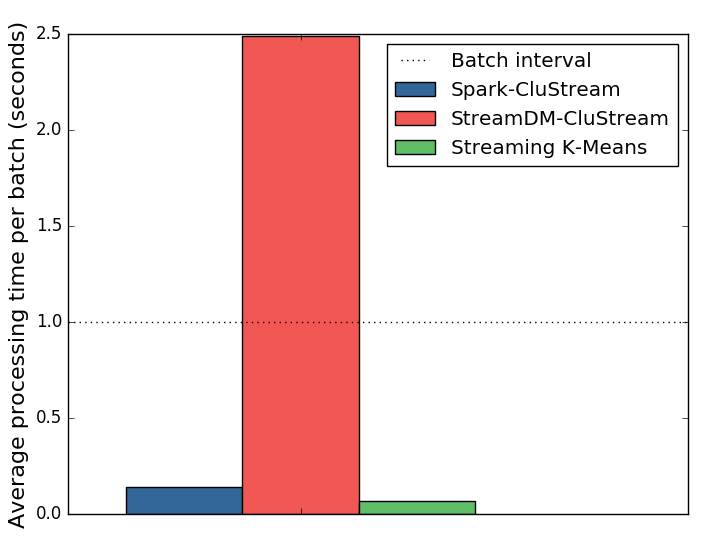
\includegraphics[scale=0.47]{./styles/singlemachine.png}
 \caption{Processing time comparison for a single machine: $q=50$, $d=34$}
 \label{fig:singlemachine}
\end{figure}

The results shown in Figure \ref{fig:singlemachine} are quite remarkable. As \textit{StreamDM-CluStream} shows a very significant disadvantage when using greater numbers of micro-clusters and higher dimensions.

For this single machine test, \textit{Spark-CluStream} was about 18 times faster on average than \textit{StreamDM-CluStream} and about two times slower than \textit{Streaming K-Means} on average.

Another consideration to be made, is that  \textit{Spark-CluStream} saves a snapshot for every batch of data, having to write to disk, while the other two algorithms never access the disk or this matter.




%-------------------------------------------------------------
\section{Conclusions}
\label{sec:conclusions}
We proposed a variation of \emph{CluStream} tailored to Apache Spark, \our.
Our experiments show that~\our~achieves similar quality to the original approach~\cite{clustreamOrig}, while it is far more efficient.
% Also, \our~outperforms existing stream clustering implementations in SPARK.
Comparing to other stream clustering approaches in Spark, our results show that \textit{Streaming K-Means} is the fastest algorithm among the three tested (highly optimized for Spark), but it does not offer the flexibility of the online-offline clustering approaches like \textit{CluStream} that better fit evolving data streams. 
Comparing \our~to \huawei, \our~delivers more consistent and accurate results, and outperforms \huawei in most cases, including one up to around 18 times faster. 

% Our~\our~on the other hand does not only deliver qualitative clustering results, but also outperforms \textit{StreamDM}, another \emph{CluStream} implementation. 
% Quality-wise it delivered more consistent and accurate results, and performance-wise it outperformed it in most cases, including one up to around 18 times faster. 
As part of our future work, we will focus on minimizing the communication cost between the different nodes to further improve the efficiency and also on dealing with outliers to improve quality.

% Bringing successfully the \textit{CluStream} method to Spark has provided valuable information about how similar methods could be adapted by reviewing some of the challenges which might occur. It has also provided deep understanding of this method itself and how stream clustering differs from other clustering methods, which might not need to adapt to changing data, of Apache Spark and how distributed systems work in general, but most importantly it has provided the experience to parallelize algorithms for the specific requirements of a given problem and this knowledge itself is applicable to an uncountable number of problems.


% \subsection{Goals achieved}

% It is rewarding to conclude that the goals were met satisfactorily. Here, the conclusions for every one of them.

% \subsubsection{Adapt \textit{CluStream} in Spark (Spark-CluStream)}

% This is the main goal of this thesis, and none of the other goals would have been met if this one failed. Adapting \textit{CluStream} in Spark brought many challenges: one being the fact that the streaming library in Spark handles streams as batches and not individual points with time stamps, forcing this adaptation to change a few things that differentiate it from the original method, and the other one being the parallelization of the algorithm in order to take advantage of distributed computing.

% Even though this adaptation changed the way data is processed, i.e. processing the stream in batches of data in parallel as much as possible, the results indicate that this was done correctly: it showed that it is not only capable of correctly clustering streams of data but it was able to match the quality of the original method described in \cite{clustreamOrig}. It was shown for two different scenarios that this is true, when comparing the errors obtained after replicating the tests done by the authors of \textit{CluStream}.

% \subsubsection{Understanding its advantages and disadvantages}

% The second most important goal was to make this adaptation as scalable as possible, and for this reason many tests were made using different scenarios. There are clearly cases where it is not fully scalable, but for the most part it was shown comparable scalability as some of the alternatives for Spark, including a method native of Spark and a similar method developed by a team from \textit{Huawei} for a set of stream mining algorithms called \textit{StreamDM}.

% Some of its limitations were also understood , such as bottlenecks that might reduce the scalability and performance in general, such as:

% \begin{itemize}
%  \item Outliers: handling with outliers in sequential code is expected to be a bottleneck, depending on the stream, a batch of data might contain points which do not belong to any micro-cluster and therefore, they have to be handled differently. Depending on the number of outliers, in particular the ones which require two micro-clusters to be merged, the total processing time for that batch will be affected negatively. In general there are three situations where this would normally occur: at the beginning of the stream if the initialization is not accurate, when the incoming data is very noisy and when the data dramatically changes.
%  \item Communication costs: running in parallel requires certain communication between processing units. This affects the scalability negatively when few computations are required and too many processing units are used, as most of the time will be spent on communication. Also, even when it is expected to be scalable, increasing the number of micro-clusters used and the dimensionality of the data results in a bigger amount of information to communicate, and therefore not allowing greater speedups after a certain amount of processing units. 
% \end{itemize}



\nocite{*}
\bibliography{literature.bib}
\bibliographystyle{plain}

\end{document}


